%% Author: Leighton Pritchard
%% Copyright: James Hutton Institute
%% 2015-03-07: Slides for teaching at University of Dundee, 17th March 2015
%% This presentation was an invited lecture on comparative genomics and visualisation
%% for the BS32010 course.

%% UNCOMMENT FOR SLIDES
\documentclass[table]{beamer}
\mode<presentation>

%% UNCOMMENT FOR HANDOUTS
%\documentclass[handout]{beamer}
\usepackage{handoutWithNotes}
\pgfpagesuselayout{4 on 1 with notes}[a4paper,border shrink=5mm]

%% GENERIC STYLE SETTINGS BELOW
\usetheme{default}
\usepackage{listings}
\usepackage{multirow}
\usepackage{xcolor}
\usepackage{hyperref}
%\usepackage[multiple]{footmisc}

\usebackgroundtemplate{

\includegraphics[width=\paperwidth,height=\paperheight]{images/hutton_background}
}
%% PRESENTATION CONFIGURATION PARAMETERS %%%%%%%%%%%%%%%%%%%%%%%%%%%%%%%%%%%%%%%
%\titlebackgroundfile{images/hutton_title}
%\framebackgroundfile{images/hutton_background}
\definecolor{hutton_green}{HTML}{78A22F}
\definecolor{hutton_purple}{HTML}{872175}
\definecolor{hutton_blue}{HTML}{569BBE}
\definecolor{olive}{rgb}{0.3, 0.4, .1}
\definecolor{fore}{RGB}{249,242,215}
\definecolor{back}{RGB}{51,51,51}
\definecolor{title}{RGB}{255,0,90}
\definecolor{dgreen}{rgb}{0.,0.6,0.}
\definecolor{gold}{rgb}{1.,0.84,0.}
\definecolor{JungleGreen}{cmyk}{0.99,0,0.52,0}
\definecolor{BlueGreen}{cmyk}{0.85,0,0.33,0}
\definecolor{RawSienna}{cmyk}{0,0.72,1,0.45}
\definecolor{Magenta}{cmyk}{0,1,0,0}
\usefonttheme{structurebold}
\setbeamercolor{alerted text}{fg=orange}
\setbeamercolor{background canvas}{bg=white}
\setbeamercolor{block title}{bg=hutton_purple}
\setbeamercolor{frametitle}{fg=hutton_purple}
\setbeamercolor{title}{fg=black}
\setbeamercolor{titlelike}{fg=hutton_green}
\setbeamercolor{author}{fg=hutton_purple}
\setbeamercolor{author in head/foot}{fg=white}
\setbeamercolor{title in head/foot}{fg=white}
\setbeamercolor{section in head/foot}{fg=hutton_purple}
\setbeamercolor{normal text}{fg=black}
\setbeamercolor{frametitle}{fg=hutton_purple}
\setbeamerfont{block title}{size={}}
\setbeamerfont{author}{size=\footnotesize}
\setbeamerfont{institute}{size=\tiny}
\setbeamerfont{date}{size=\footnotesize}
\setbeamercolor{section in toc shaded}{fg=hutton_purple}
\setbeamercolor{section in toc}{fg=hutton_purple}
\setbeamercolor{subsection in toc shaded}{fg=hutton_purple}
\setbeamercolor{subsection in toc}{fg=hutton_purple}
\setbeamertemplate{itemize item}[circle]
\setbeamertemplate{itemize subitem}[circle]
\setbeamertemplate{itemize subsubitem}[circle]
\setbeamertemplate{itemize subsubsubitem}[circle]
\setbeamercolor{itemize item}{fg=hutton_purple}
\setbeamercolor{itemize subitem}{fg=hutton_purple}
\setbeamercolor{itemize subsubitem}{fg=hutton_purple}
\setbeamercolor{itemize subsubsubitem}{fg=hutton_purple}
\setbeamercolor{enumerate item}{fg=hutton_purple}
\setbeamercolor{enumerate subitem}{fg=hutton_purple}
\setbeamercolor{enumerate subsubitem}{fg=hutton_purple}
\setbeamercolor{enumerate subsubsubitem}{fg=hutton_purple}
\setbeamercolor{alerted text}{fg=hutton_green}
\setbeamerfont{alerted text}{series=\bfseries}
% This command makes sure that acrobat reader doesn't change the colours of the slide
% when there are figures with transparencies.
\pdfpageattr {/Group << /S /Transparency /I true /CS /DeviceRGB>>}

%Disables discrete bottom navigation bar
\beamertemplatenavigationsymbolsempty

% Modify the slide titles to avoid the corner images,
\setbeamertemplate{frametitle}
{
\vspace{0.05\textheight}
\noindent\quad\begin{minipage}[t][0.12\textheight][t]{0.85\textwidth}
\insertframetitle\par
\end{minipage}
}

% Modify title page to avoid the big logo on right
\setbeamertemplate{title page}{
    \begin{picture}(0,0)
            %This ends up on top of the default background image, rather than replacing it:
            \put(-30,-165){%
                
\includegraphics[width=\paperwidth,height=\paperheight]{images/hutton_title}
            }
            \put(0,-75){%
                \begin{minipage}[b][0.4\textheight][t]{0.75\textwidth}
                    \usebeamerfont{title}\usebeamercolor[fg]{title}{\inserttitle\par}
                    \usebeamerfont{subtitle}\usebeamercolor[fg]{subtitle}{\insertsubtitle\par}
                \end{minipage}
            }
            \put(0,-125){%
                \begin{minipage}[b][0.1\textheight][t]{\textwidth}
                    \usebeamerfont{author}\usebeamercolor[fg]{author}{\insertauthor\par}
                    \usebeamerfont{institute}\usebeamercolor[fg]{institute}{\insertinstitute\par}
                \end{minipage}
            }
    \end{picture}
}

% Make \verbatim environment tiny font
\makeatletter
\def\verbatim{\tiny\@verbatim \frenchspacing\@vobeyspaces \@xverbatim}
\makeatother

%%%%%%%%%%%%%%%%%%%%%%%%%%%%%%%%%%%%%%%%%%%%%%%%%%%%%%%%%%%%%%%%%%%%%%%%%%%%%%%%

% LISTINGS SETTING
% Settings for code listings in lstlistings

\definecolor{hutton_lightgreen}{HTML}{C8F27F}

\lstset{ %
  backgroundcolor=\color{hutton_lightgreen},   % choose the background color; you must add \usepackage{color} or \usepackage{xcolor}
  basicstyle=\tiny\ttfamily,        % the size of the fonts that are used for the code
  breakatwhitespace=false,         % sets if automatic breaks should only happen at whitespace
  breaklines=true,                 % sets automatic line breaking
  captionpos=b,                    % sets the caption-position to bottom
  commentstyle=\color{red},    % comment style
  deletekeywords={...},            % if you want to delete keywords from the given language
  escapeinside={\%*}{*)},          % if you want to add LaTeX within your code
  extendedchars=true,              % lets you use non-ASCII characters; for 8-bits encodings only, does not work with UTF-8
  frame=single,                    % adds a frame around the code
  keepspaces=true,                 % keeps spaces in text, useful for keeping indentation of code (possibly needs columns=flexible)
  keywordstyle=\color{blue},       % keyword style
%  language=Octave,                 % the language of the code
  morekeywords={*,...},            % if you want to add more keywords to the set
  numbers=left,                    % where to put the line-numbers; possible values are (none, left, right)
  numbersep=5pt,                   % how far the line-numbers are from the code
  numberstyle=\tiny\color{gray}, % the style that is used for the line-numbers
  rulecolor=\color{black},         % if not set, the frame-color may be changed on line-breaks within not-black text (e.g. comments (green here))
  showspaces=false,                % show spaces everywhere adding particular underscores; it overrides 'showstringspaces'
  showstringspaces=false,          % underline spaces within strings only
  showtabs=false,                  % show tabs within strings adding particular underscores
  stepnumber=1,                    % the step between two line-numbers. If it's 1, each line will be numbered
  stringstyle=\color{violet},     % string literal style
  tabsize=4,                       % sets default tabsize to 2 spaces
  title=\lstname                   % show the filename of files included with \lstinputlisting; also try caption instead of title
}


%%%
% TITLE PREAMBLE
\title[Comparative Genomics and Visualisation: 4.Genome Features] % (optional, only for long titles)
{Comparative Genomics and \\ Visualisation \\
BS32010 \\
4.Genome Feature Comparisons}
%\subtitle{}
\author[Pritchard] % (optional, for multiple authors)
{Leighton~Pritchard$^{1,2,3}$}
\institute[The James Hutton Institute] % (optional)
{
  $^{1}$Information and Computational Sciences,\\
  $^{2}$Centre for Human and Animal Pathogens in the Environment,\\
  $^{3}$Dundee Effector Consortium,\\
  The James Hutton Institute, Invergowrie, Dundee, Scotland, DD2 5DA
}
\date[17th March 2015] % (optional)
{17th March 2015}
\subject{Bioinformatics, Genomics, Bacteria, Sequencing, Microbiology, Microbes, Comparative Genomics, Visualisation}

%%%
% TOC
% Show table of contents, with current section highlighted,
% at the start of each section

%\AtBeginSection[]
%{
%  \begin{frame}
%    \frametitle{Table of Contents}
%    \tableofcontents[currentsection] %,hideallsubsections]
%  \end{frame}
%}

\AtBeginSubsection[]
{
  \begin{frame}
    \frametitle{Table of Contents}
    \tableofcontents[currentsection,currentsubsection] %,hideallsubsections]
  \end{frame}
}

%%%
% START DOCUMENT
\begin{document}

\frame[plain]{\titlepage}

%% use.tex
%% Author: Leighton Pritchard
%% Copyright: James Hutton Institute
%% These slides describe the acceptable use policy for these slides and
%% materials

%
\begin{frame}
  \frametitle{Acceptable Use Policy}
  Recording of this talk, taking photos, discussing the content using \\
  email, Twitter, blogs, etc. is permitted (and encouraged), \\
  providing distraction to others is minimised. \\[0.5cm]
  These slides will be made available on SlideShare. \\[0.5cm]
  \textbf{These slides, and supporting material including exercises, are available at \href{https://github.com/widdowquinn/Teaching-2015-03-17-UoD_compgenvis}{https://github.com/widdowquinn/Teaching-2015-03-17-UoD\_compgenvis}}
\end{frame}

%%%
% SECTION: Comparisons of genome Features
\section{Comparisons of genome features}
% SUBSECTION
% Genome features
\subsection{Genome Features}
%% genome_features.tex
%% Author: Leighton Pritchard
%% Copyright: James Hutton Institute
%% Genome features

%
\begin{frame}
  \frametitle{Gene features}
  \textcolor{hutton_green}{Genes:}
  \begin{columns}[T] 
    \column{.4\textwidth} 
      \begin{itemize}
        \item translation start
        \item introns
        \item exons
        \item translation stop
        \item translation terminator
      \end{itemize}
    \column{.6\textwidth}
      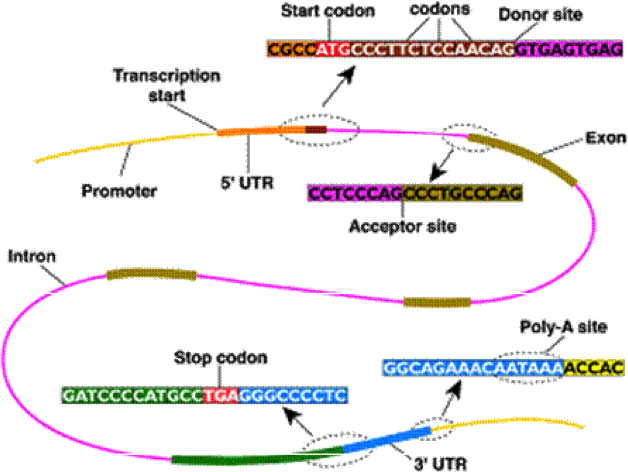
\includegraphics[width=\textwidth]{images/gene_feature}
  \end{columns}    
\end{frame}

%
\begin{frame}
  \frametitle{RNA features}
  \textcolor{hutton_blue}{RNA/ncRNA: characterised by complex secondary structure}
  \begin{columns}[T] 
    \column{.4\textwidth} 
      \begin{itemize}
        \item tRNA - transfer RNA
        \item rRNA - ribosomal RNA
        \item CRISPRs - prokaryotic defence, and genome editing
        \item many other functional classes, including enhancers
      \end{itemize}
    \column{.6\textwidth}
      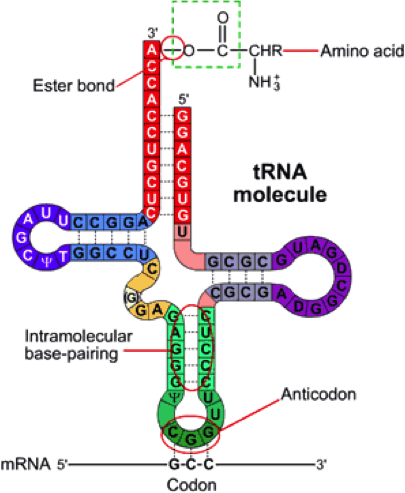
\includegraphics[height=0.7\textheight]{images/rna_feature}
  \end{columns}    
\end{frame}

%
\begin{frame}
  \frametitle{Gene features}
  \textcolor{hutton_green}{Regulatory sites:}
  \begin{itemize}
    \item transcription start sites (TSS)
    \item RNA polymerase (RNAp) binding sites
    \item transcription factor binding sites (TFBS)
    \item core, proximal and distal promoter regions
  \end{itemize}
  	
  \includegraphics[width=\textwidth]{images/_feature}
  \end{columns}    
\end{frame}

%
\begin{frame}
  \frametitle{Gene features}
  \textcolor{hutton_blue}{Genes:}
  \begin{columns}[T] 
    \column{.4\textwidth} 
      \begin{itemize}
        \item translation start
        \item introns
        \item exons
        \item translation stop
        \item translation terminator
      \end{itemize}
    \column{.6\textwidth}
      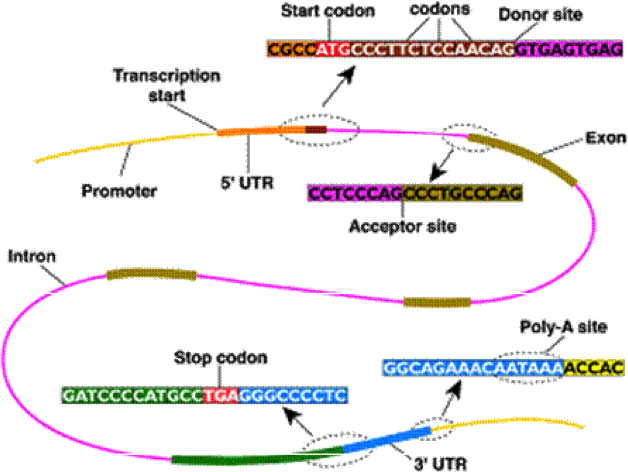
\includegraphics[width=\textwidth]{images/gene_feature}
  \end{columns}    
\end{frame}
%% feature_finding.tex
%% Author: Leighton Pritchard
%% Copyright: James Hutton Institute
%% Finding genome features

%
\begin{frame}
  \frametitle{Gene finding
  \footnote{\tiny{\href{http://dx.doi.org/10.1101/gr.088997.108
}{Liang \textit{et al.} (2009) \textit{Genome Res.} doi:10.1101/gr.088997.108
}}}
    \footnote{\tiny{\href{http://dx.doi.org/10.1038/nbt0807-883
}{Brent (2007) \textit{Nat. Biotech.} doi:10.1038/nbt0807-883
}}}
    \footnote{\tiny{\href{http://dx.doi.org/10.1186/1471-2105-5-59
}{Korf (2004) \textit{BMC Bioinf.} doi:10.1186/1471-2105-5-59
}}}
    }
  At genome scales, we need to automate functional prediction \\~\\    
  \textcolor{hutton_green}{Empirical (evidence-based) methods:}
  \begin{itemize}
    \item Inference from known protein/cDNA/mRNA/EST sequence
    \item Interference from mapped RNA reads (e.g. RNAseq)
  \end{itemize}
  \textcolor{hutton_blue}{\textit{Ab initio} methods:}
  \begin{itemize}
    \item Prediction on the basis of gene features (TSS, CpG islands, Shine-Dalgarno sequence, stop codons, nucleotide composition, etc.)
  \end{itemize}
  \textcolor{hutton_purple}{\textbf{Inference from genome comparisons/sequence conservation}}
\end{frame}

%
\begin{frame}
  \frametitle{Regulatory element finding
  \footnote{\tiny{\href{http://dx.doi.org/10.1186/1471-2105-12-238
}{Zhang \textit{et al.} (2011) \textit{BMC Bioinf.} doi:10.1186/1471-2105-12-238
}}}
    \footnote{\tiny{\href{http://dx.doi.org/10.1093/nar/gkt1123
}{Kilic \textit{et al.} (2013) \textit{Nucl. Acids Re.} doi:10.1093/nar/gkt1123
}}}
    \footnote{\tiny{\href{http://dx.doi.org/10.1016/j.gde.2005.05.002
}{Vavouri \& Elgar (2005) \textit{Curr. Op. Genet. Deve.} doi:10.1016/j.gde.2005.05.002
}}}
    }
  \textcolor{hutton_green}{Empirical (evidence-based) methods:}
  \begin{itemize}
    \item Inference from protein-DNA binding experiments
    \item Interference from co-expression
  \end{itemize}
  \textcolor{hutton_blue}{\textit{Ab initio} methods:}
  \begin{itemize}
    \item Identification of regulatory motifs (profile/other methods; TATA, $\sigma$-factor binding sites, etc.)
    \item Statistical overrepresentation of motifs
    \item Identification from sequence properties
  \end{itemize}
  \textcolor{hutton_purple}{\textbf{Inference from genome comparisons/sequence conservation}}
\end{frame}

%
\begin{frame}
  \frametitle{Multiple genome alignment}
  \Large{
    \textcolor{hutton_blue}{
      \textbf{
      EXERCISE 7: \\
      {\small \href{https://github.com/widdowquinn/Teaching-2015-03-17-UoD_compgenvis/blob/master/exercises/predict_CDS/bacterial_CDS_prediction.md}{\texttt{predict\_CDS/bacterial\_CDS\_prediction.md}}}
      }
    }
  }
\end{frame}

%
\begin{frame}
  \frametitle{Genecalling software}
  \textcolor{hutton_green}{Many options for this, including$\ldots$}
  \textcolor{hutton_blue}{Prokaryotes}
  \begin{itemize}
    \item Glimmer: {\tiny\href{http://ccb.jhu.edu/software/glimmer/index.shtml}{http://ccb.jhu.edu/software/glimmer/index.shtml}}
    \item GeneMarkS: {\tiny\href{http://opal.biology.gatech.edu/}{http://opal.biology.gatech.edu/}}
    \item RAST: {\tiny\href{http://rast.nmpdr.org/}{http://rast.nmpdr.org/}}
    \item BASys: {\tiny\href{https://www.basys.ca/}{https://www.basys.ca/}}
    \item \textbf{Prokka: {\tiny\href{http://www.vicbioinformatics.com/software.prokka.shtml}{http://}www.vicbioinformatics.com/software.prokka.shtml}}
  \end{itemize}
  \textcolor{hutton_purple}{Eukaryotes}
  \begin{itemize}
    \item GlimmerHMM: {\tiny\href{http://ccb.jhu.edu/software/glimmerhmm/}{http://ccb.jhu.edu/software/glimmerhmm/}}
    \item GeneMarkES: {\tiny\href{http://opal.biology.gatech.edu/gmseuk.html}{http://opal.biology.gatech.edu/gmseuk.html}}
    \item Augustus: {\tiny\href{http://augustus.gobics.de/}{http://augustus.gobics.de/}}
    \item SNAP: {\tiny\href{http://korflab.ucdavis.edu/software.html}{http://korflab.ucdavis.edu/software.html}}
  \end{itemize}
\end{frame}

%
\begin{frame}
  \frametitle{Feature identification}
  \textcolor{hutton_green}{All prediction methods give you errors}
  \begin{itemize}
    \item \textbf{False positive}: predicts features where there are none
    \item \textbf{False negative}: fails to predict a feature that is present
    \item \textbf{Magnitude}: does not identify correct bounds on/value for feature
    \item \textbf{Category}: predicts a feature to belong to the wrong class
  \end{itemize}
  \textcolor{hutton_blue}{All experiments have errors} \\~\\
  \textcolor{hutton_purple}{\textbf{Genome comparisons can help correct for these errors}}
\end{frame}
% SUBSECTION
% Who let the -logues out?
\subsection{Who Let the -logues Out?}
%% equivalent_genome_features.tex
%% Author: Leighton Pritchard
%% Copyright: James Hutton Institute
%% A brief description of genome feature prediction, and related
%% issues

% What do you align, and why?
\begin{frame}
  \frametitle{What makes genome features equivalent?}
  \begin{center}
    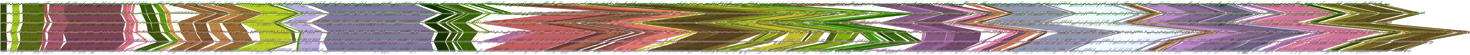
\includegraphics[width=1\textwidth]{images/collinear_zeae}  
  \end{center}
  When we compare two features (e.g. genes) between two or more genomes, there must be some basis for making the comparison \\
  That is, they have to be \textit{equivalent} in some way, such as:
  \begin{itemize}
    \item common evolutionary origin
    \item functional similarity
    \item a family-based relationship
  \end{itemize}
  It's common to define equivalence of genome features in terms of evolutionary relationship.
\end{frame}

% What do you align, and why?
\begin{frame}
  \frametitle{Why look at equivalent features?}
  \begin{center}
    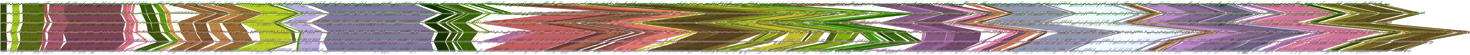
\includegraphics[width=1\textwidth]{images/collinear_zeae}  
  \end{center}
  \textbf{The real power of genomics is comparative genomics!}
  \begin{itemize}
    \item Makes catalogues of genome components comparable between organisms
    \item Differences, e.g. presence/absence of equivalents may support hypotheses for functional or phenotypic difference
    \item Can identify characteristic signals for diagnosis/epidemiology
    \item Can build parts lists and wiring diagrams for systems and synthetic biology
  \end{itemize}
\end{frame}

%% logues.tex
%% Author: Leighton Pritchard
%% Copyright: James Hutton Institute
%% Who let the -logues out?

%
\begin{frame}
  \frametitle{Who let the -logues out?}
  \Large{
    \textcolor{olive}{
      \textbf{
      Genome features can have complex evolutionary relationships \\~\\
      We need precise terms to describe these relationships
      }
    }
  }
  \begin{center}
    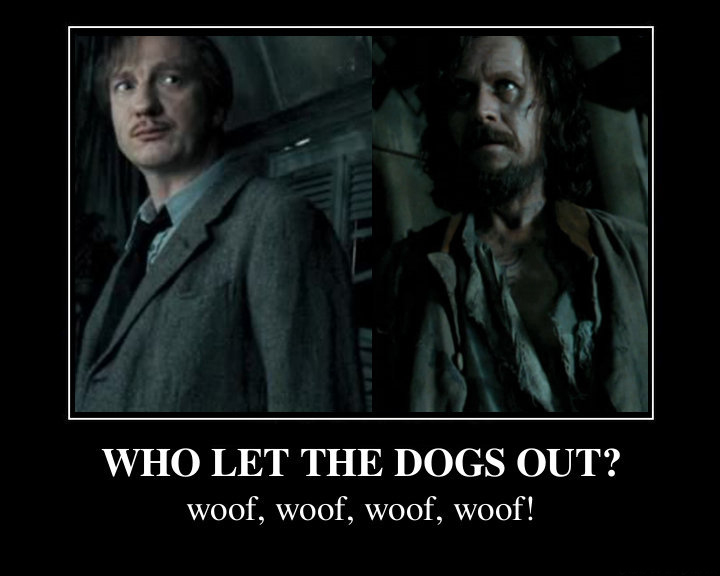
\includegraphics[width=0.4\textwidth]{images/who_let_the_dogs_out}
  \end{center}      
\end{frame}

%
\begin{frame}
  \frametitle{The -logues drop
  \footnote{\tiny{\href{http://dx.doi.org/10.2307/2412448
}{Fitch \textit{et al.} (1970) \textit{Syst. Zool.} doi:10.2307/2412448
}}}
  }
  How do we understand the relationships between features in more than one genome?
  \begin{itemize}
    \item \textcolor{hutton_green}{Functional similarity}: \textbf{analogy}
    \item \textcolor{hutton_blue}{Evolutionary common origin}: \textbf{homology, orthology, etc.}
    \item \textcolor{hutton_purple}{Evolutionary/functional/family relationship}: \textbf{paralogy}
  \end{itemize}
  \begin{center}
    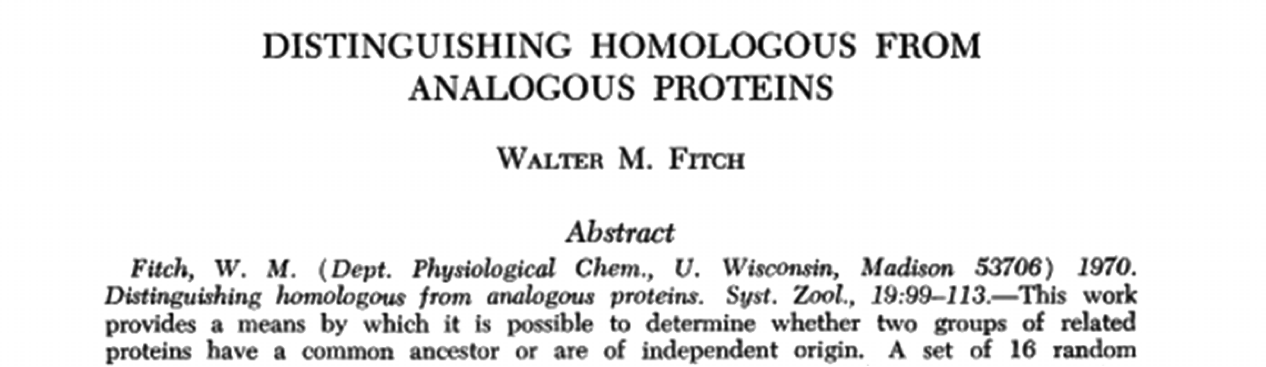
\includegraphics[width=\textwidth]{images/fitch}
  \end{center}    
\end{frame}

%
\begin{frame}
  \frametitle{Definitions
  }
  Technical terms describing evolutionary relationships
  \begin{itemize}
    \item \textbf{\textcolor{hutton_blue}{Homologues}}: share a common ancestor \textcolor{red}{\textbf{NOTE: there are NOT degrees of homology}}
    \item \textbf{\textcolor{hutton_blue}{Analogues}}: are functionally similar. Analogues may or may not share common ancestry
    \item \textbf{\textcolor{hutton_green}{Orthologues}}: are homologues that \textit{diverged through speciation}
    \item \textbf{\textcolor{hutton_purple}{Paralogues}}: are homologues that \textit{diverged through duplication} within the same genome
  \end{itemize}
  (also \textit{co-orthologues}, \textit{xenologues}, etc.)
\end{frame}
% SUBSECTION
% What's so important about orthologues
\subsection{What's so important about orthologues?}
%% orthologue_conjecture.tex
%% Author: Leighton Pritchard
%% Copyright: James Hutton Institute
%% A brief introduction to orthologues, and their prediction

%
\begin{frame}
  \frametitle{The Ortholog Conjecture
    \footnote{\tiny{Nehrt \textit{et al.} (2011) \textit{PLoS Comp. Biol.} \href{http://dx.doi.org/10.1371/journal.pcbi.1002073}{doi:10.1371/journal.pcbi.1002073
    }}}  
    \footnote{\tiny{Chen \textit{et al.} (2012) \textit{PLoS Comp. Biol.} \href{http://dx.doi.org/10.1371/journal.pcbi.1002784}{doi:10.1371/journal.pcbi.1002784
    }}}  
  }
  \Large{
    \textcolor{olive}{
      \textbf{
      Without duplication, a gene product is unlikely to change its basic function, because this would lead to loss of the original function, and this would be harmful.
      }
    }
  }
\end{frame}

%
\begin{frame}
  \frametitle{The Ortholog Conjecture
    \footnote{\tiny{Nehrt \textit{et al.} (2011) \textit{PLoS Comp. Biol.} \href{http://dx.doi.org/10.1371/journal.pcbi.1002073}{doi:10.1371/journal.pcbi.1002073
    }}}  
  }
  \begin{itemize}
    \item Paralogues are better predictors of function than orthologues \\
      \textcolor{red}{$\therefore$ the conjecture is false}
    \item Cellular context is better for protein function inference
  \end{itemize}
  \textcolor{hutton_green}{(function defined in Gene Ontology (GO) terms)}
    \begin{center}
      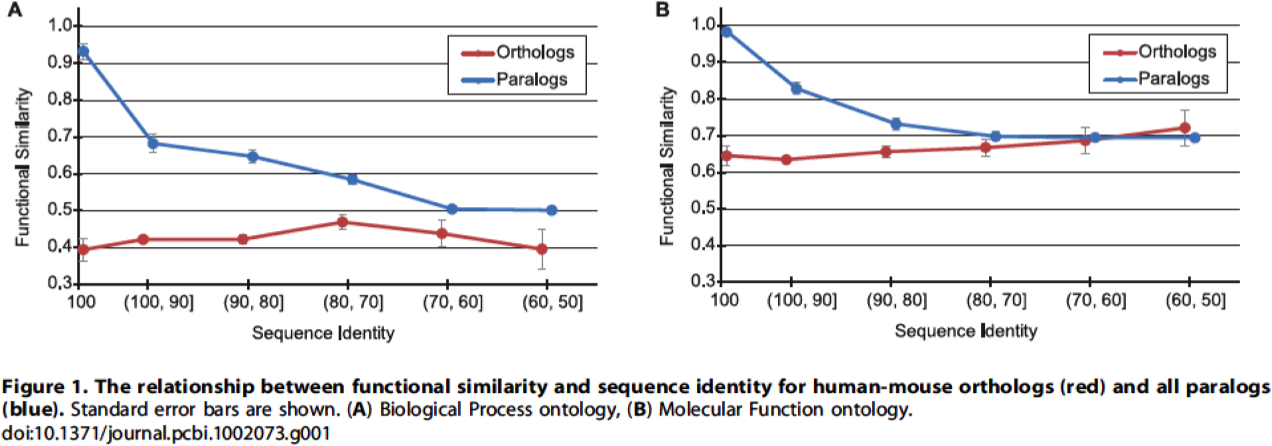
\includegraphics[width=\textwidth]{images/nehrt_orthologues}      
    \end{center}  
\end{frame}

%
\begin{frame}
  \frametitle{The Ortholog Conjecture
    \footnote{\tiny{Chen \textit{et al.} (2012) \textit{PLoS Comp. Biol.} \href{http://dx.doi.org/10.1371/journal.pcbi.1002784}{doi:10.1371/journal.pcbi.1002784
    }}}  
  }
  \textcolor{hutton_green}{We do not understand function well enough to test the conjecture}
  \begin{itemize}
    \item ``examination of functional studies of homologs with identical protein sequences reveals \textcolor{red}{experimental biases, annotation errors, and homology-based functional inferences that are labeled in GO as experimental}. These problems [$\ldots$] make the current GO inappropriate for testing the ortholog conjecture''
    \item Expression level similarity is more similar for orthologues than paralogues \\
    \textcolor{hutton_blue}{(but is this function?)}
  \end{itemize}
\end{frame}
%% orthologue_prediction.tex
%% Author: Leighton Pritchard
%% Copyright: James Hutton Institute
%% A brief introduction to orthologues, and their prediction

% 
\begin{frame}
  \frametitle{Why focus on orthologues?
    \footnote{\tiny{Chen and Zhang (2012) \textit{PLoS Comp. Biol.} \href{http://dx.doi.org/10.1371/journal.pcbi.1002784}{doi:10.1371/journal.pcbi.1002784
    }}}  
    \footnote{\tiny{Dessimoz (2011) \textit{Brief. Bioinf.} \href{http://dx.doi.org/10.1093/bib/bbr057}{doi:10.1093/bib/bbr057
    }}}
    \footnote{\tiny{Altenhoff and Dessimoz (2009) \textit{PLoS Comp. Biol.} \textbf{5}:e1000262 \href{http://dx.doi.org/10.1371/journal.pcbi.1000262}{doi:10.1371/journal.pcbi.1000262
    }}}
  }
  Formalisation of the idea of \textit{corresponding genes} in different organisms. \\
  \textcolor{hutton_blue}{Orthologues serve two purposes:}
  \begin{itemize}
    \item \textcolor{hutton_green}{\textbf{Evolutionary equivalence}}
    \item \textcolor{hutton_purple}{\textbf{Functional equivalence}} (``The Ortholog Conjecture'')
  \end{itemize}
  Applications in comparative genomics, functional genomics and phylogenetics. \\
  \textcolor{RawSienna}{Over 30 databases attempt to describe orthologous relationships} (\href{http://questfororthologs.org/orthology_databases
}{http://questfororthologs.org/orthology\_databases})
\end{frame}

%
\begin{frame}
  \frametitle{Finding ``Orthologues''}
  \Large{
    \textcolor{olive}{
      \textbf{
      The process of finding evolutionary (and/or) functional equivalents of genes across two or more organisms's genomes
      }
    }
  }
\end{frame}

% Orthologue-finding methods
\begin{frame}
  \frametitle{Finding orthologues
    \footnote{\tiny{Kristensen \textit{et al}. (2011) \textit{Brief. Bioinf.} \textbf{12}:379-391 \href{http://dx.doi.org/10.1093/bib/bbr030}{doi:10.1093/bib/bbr030
    }}}
    \footnote{\tiny{Trachana \textit{et al}. (2011) \textit{Bioessays} \textbf{33}:769-780 \href{http://dx.doi.org/10.1002/bies.201100062}{doi:10.1002/bies.201100062
    }}}
    \footnote{\tiny{Salichos and Rokas (2011) \textit{PLoS One} \textbf{6}:e18755 \href{http://dx.doi.org/10.1371/journal.pone.0018755.g006}{doi:10.1371/journal.pone.0018755.g006
    }}}
  }
  Multiple methods and databases
  \begin{columns}[T]    \begin{column}{6cm}
      \begin{itemize}
        \item \textcolor{hutton_green}{\textbf{Pairwise genome}}
        \begin{itemize}
          \item \href{http://armchairbiology.blogspot.co.uk/2012/07/on-reciprocal-best-blast-hits.html}{RBBH} (aka BBH, RBH), \href{http://link.springer.com/protocol/10.1007/978-1-59745-515-2_7}{RSD}, \href{http://inparanoid.sbc.su.se/cgi-bin/index.cgi}{InParanoid}, \href{http://roundup.hms.harvard.edu/}{RoundUp}
        \end{itemize}
        \item \textcolor{hutton_blue}{\textbf{Multi-genome}}
        \begin{itemize}
          \item \textit{Graph-based}: \href{http://www.ncbi.nlm.nih.gov/COG/}{COG}, \href{http://eggnog.embl.de/}{eggNOG}, \href{http://cegg.unige.ch/orthodb7}{OrthoDB}, \href{http://orthomcl.org/orthomcl/}{OrthoMCL}, \href{http://omabrowser.org/cgi-bin/gateway.pl}{OMA}, \href{http://multiparanoid.sbc.su.se/}{MultiParanoid}
          \item \textit{Tree-based}: \href{http://www.treefam.org/}{TreeFam}, \href{http://www.ensembl.org/info/genome/compara/index.html}{Ensembl Compara}, \href{http://phylomedb.org/}{PhylomeDB}, \href{https://trac.nbic.nl/loft/}{LOFT}
        \end{itemize}
      \end{itemize}
    \end{column}
    \begin{column}{4cm}
      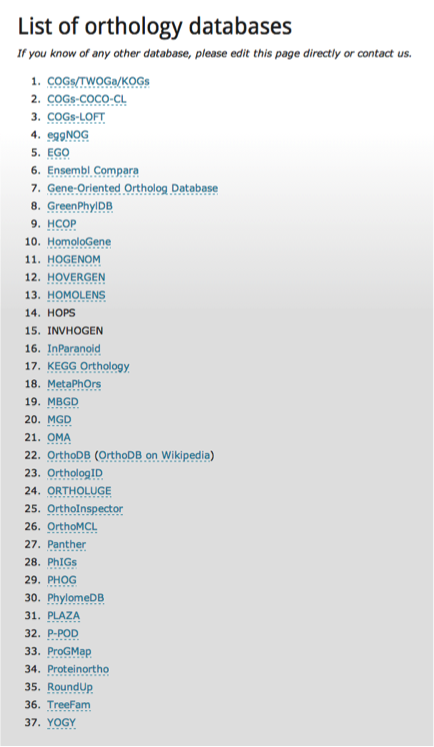
\includegraphics[height=0.575\textheight]{images/orthology_databases}      
    \end{column}
  \end{columns}
\end{frame}


%% rbbh.tex
%% Author: Leighton Pritchard
%% Copyright: James Hutton Institute
%% An outline of the RBBH method

% Which methods work best
\begin{frame}
  \frametitle{Reciprocal Best BLAST Hits
    \footnote{\tiny\href{http://armchairbiology.blogspot.co.uk/2012/07/on-reciprocal-best-blast-hits.html}{On Reciprocal Best BLAST Hits 19/7/2012
    }}
  }
  \begin{center}
      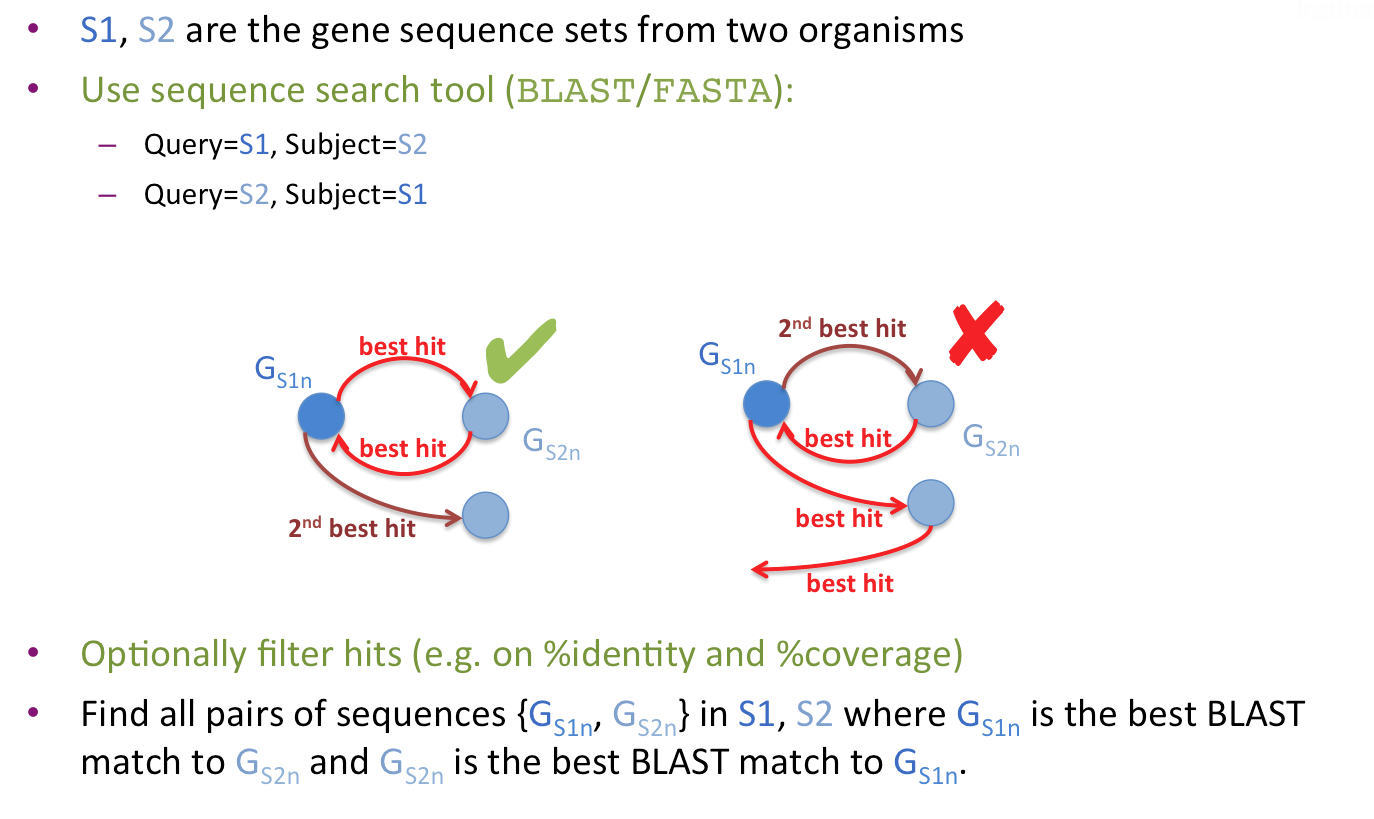
\includegraphics[width=1\textwidth]{images/rbbh}      
  \end{center}
\end{frame}

%
\begin{frame}
  \frametitle{Finding ``Orthologues'': RBBH}
  \Large{
    \textcolor{hutton_blue}{
      \textbf{
      EXERCISE 8: \\
      \texttt{ex08\_find\_rbbh.ipynb}
      }
    }
  }
\end{frame}
%% mcl.tex
%% Author: Leighton Pritchard
%% Copyright: James Hutton Institute
%% An outline of using MCL for orthologue finding

% 
\begin{frame}
  \frametitle{MCL
    \footnote{\tiny{Enright \textit{et al.} (2002) \textit{Nucl. Acids Res.} \href{http://dx.doi.org/10.1093/nar/30.7.1575}{doi:10.1093/nar/30.7.1575
    }}}
  }
  \begin{itemize}
    \item MCL constructs a network (\textit{graph}) from all-against-all BLAST results
    \item \textcolor{hutton_green}{Matrix operations (\textit{expansion}, \textit{inflation}) are applied}
    \item \textcolor{hutton_blue}{Expansion, inflation iterated until the network converges}
  \end{itemize}
  \begin{center}
      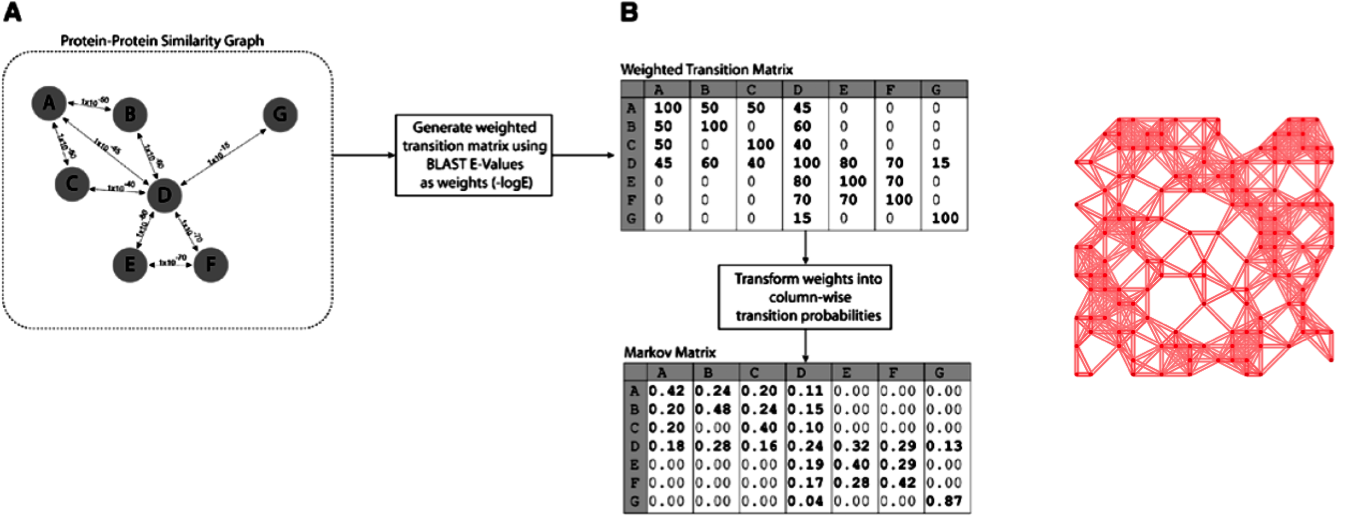
\includegraphics[width=1\textwidth]{images/mcl_intro}
  \end{center}
\end{frame}

% 
\begin{frame}
  \frametitle{MCL
    \footnote{\tiny{Enright \textit{et al.} (2002) \textit{Nucl. Acids Res.} \href{http://dx.doi.org/10.1093/nar/30.7.1575}{doi:10.1093/nar/30.7.1575
    }}}
  }  
  \begin{center}
      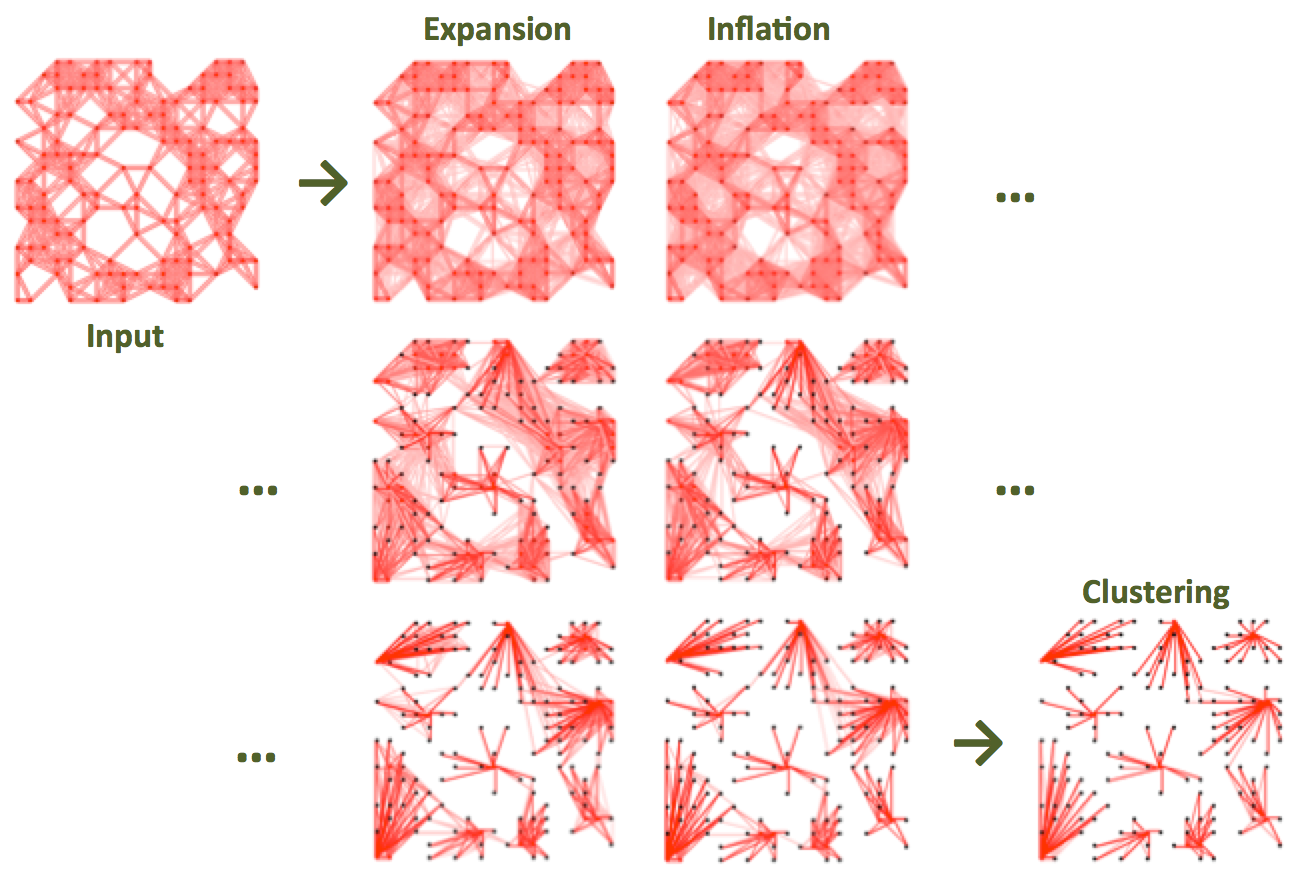
\includegraphics[width=1\textwidth]{images/mcl_method}
  \end{center}
\end{frame}

% 
\begin{frame}
  \frametitle{OrthoMCL
    \footnote{\tiny{Li \textit{et al.} (2003) \textit{Genome Res.} \href{http://dx.doi.org/10.1101/gr.1224503
}{doi:10.1101/gr.1224503
    }}}
    \footnote{\tiny \href{http://orthomcl.org/orthomcl/}{http://orthomcl.org/orthomcl/}
    }
  }
  \begin{itemize}
    \item Defines potential inparalogue, orthologue and co-orthologue pairs, \textcolor{red}{using RBBH}
    \item \textcolor{hutton_green}{Applies MCL to cluster these pairs of sequences}
    \item \textcolor{hutton_blue}{Output clusters include both orthologues and paralogues}
  \end{itemize}  
  \begin{center}
      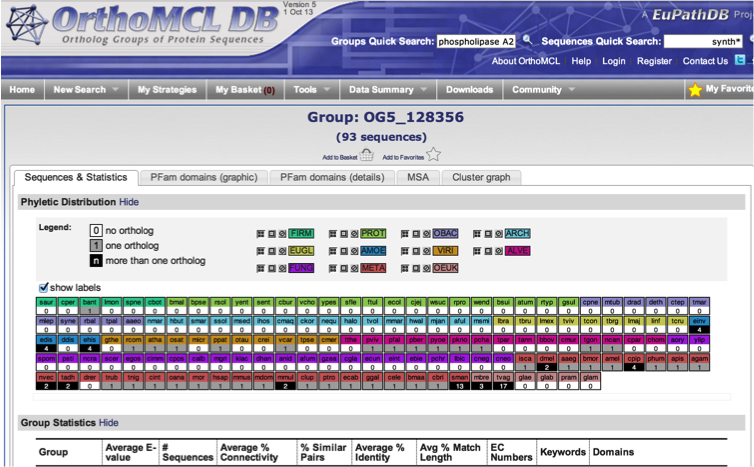
\includegraphics[width=0.7\textwidth]{images/orthomcl}
  \end{center}
\end{frame}

%
\begin{frame}
  \frametitle{Finding ``Orthologues'': MCL}
  \Large{
    \textcolor{hutton_blue}{
      \textbf{
      EXERCISE 9: \\
      {\small \href{https://github.com/widdowquinn/Teaching-2015-03-17-UoD_compgenvis/blob/master/exercises/mcl_orthologues/ex09a_mcl_orthologues.md}{\texttt{mcl\_orthologues/ex\_09a\_mcl\_orthologues.md}} \\
      \texttt{mcl\_orthologues/ex09b\_mcl\_orthologues.ipynb}}
      }
    }
  }
\end{frame}
%% other_orthologue_methods.tex
%% Author: Leighton Pritchard
%% Copyright: James Hutton Institute
%% Summary of other orthologue prediction methods

% 
\begin{frame}
  \frametitle{Notes of caution}
  \textcolor{hutton_green}{BLAST-based orthology methods are fast!} \\
  $\ldots$but there are some drawbacks:
  \begin{itemize}
    \item No guarantee that sequence matches are transitive \\
    (A may match B at a different domain that B matches C)
    \item \textcolor{hutton_blue}{No evolutionary distance model}
    \item \textcolor{hutton_purple}{Do not account for multiple domain matches}
  \end{itemize}
  Orthologues are proposed on the basis of sequence similarity, \textcolor{red}{\textbf{not predicted directly}}.
\end{frame}

% 
\begin{frame}
  \frametitle{Orthologue prediction methods}
  \textcolor{hutton_green}{Homologene (NCBI): \textit{synteny}}
  \begin{itemize}
    \item \href{http://www.ncbi.nlm.nih.gov/homologene}{http://www.ncbi.nlm.nih.gov/homologene}
  \end{itemize}
  \textcolor{hutton_blue}{Mouse Genome Database (MGD): \textit{manual curation}}
  \begin{itemize}
    \item \href{http://www.informatics.jax.org/homology.shtml}{http://www.informatics.jax.org/homology.shtml}
  \end{itemize}
  \textcolor{RawSienna}{EnsembleCompara (EMBL-EBI): \textit{tree-based}}
  \begin{itemize}
    \item \href{http://www.ensembl.org/info/genome/compara/index.html}{http://www.ensembl.org/info/genome/compara/index.html}
  \end{itemize}
  \textcolor{olive}{TreeFam (EMBL-EBI): \textit{tree-based}}
  \begin{itemize}
    \item \href{http://www.treefam.org}{http://www.treefam.org}
  \end{itemize}
  \textcolor{hutton_purple}{OrthologID: \textit{tree-based}}
  \begin{itemize}
    \item \href{http://nypg.bio.nyu.edu/orthologid}{http://nypg.bio.nyu.edu/orthologid}
  \end{itemize}
\end{frame}
%% evaluating_orthologue_prediction.tex
%% Author: Leighton Pritchard
%% Copyright: James Hutton Institute
%% A brief introduction to orthologues, and evaluation of their prediction

% SUBSECTION: Why orthologues?
\subsection{Evaluating orthologue prediction}

% Which methods work best
\begin{frame}
  \frametitle{Which prediction methods work best?
    \footnote{\tiny{Wolf and Koonin (2012) \textit{Genome Biol. Evol.} \textbf{4}:1286-1294 \href{http://dx.doi.org/10.1093/gbe/evs100}{doi:10.1093/gbe/evs100
    }}}
  }
  Taking advantage of prokaryotic operon structure: \textcolor{RawSienna}{\textbf{if the outer pair of a syntenic triplet of genes are orthologous, the middle gene is also likely to be orthologous}.}\\
  Specifically testing reciprocal best hits (RBH).
  \begin{center}
      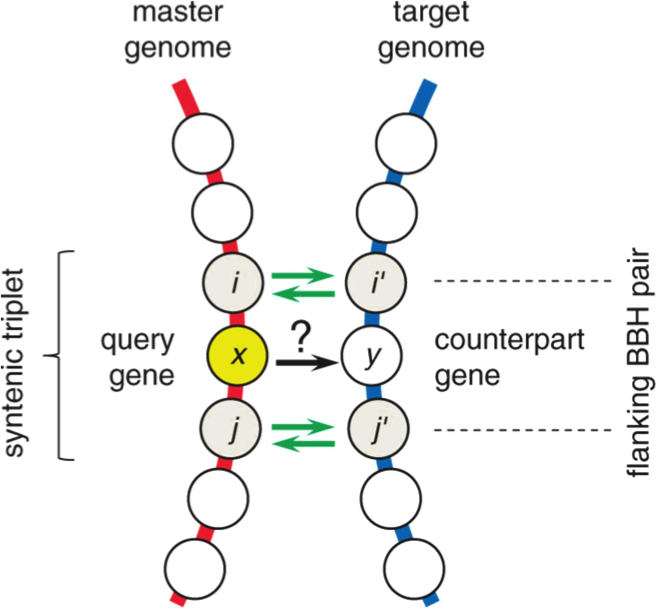
\includegraphics[height=0.45\textheight]{images/syntenic_triplet} 
  \end{center}
\end{frame}

% Which methods work best
\begin{frame}
  \frametitle{Which prediction methods work best?
    \footnote{\tiny{Wolf and Koonin (2012) \textit{Genome Biol. Evil.} \textbf{4}:1286-1294 \href{http://dx.doi.org/10.1093/gbe/evs100}{doi:10.1093/gbe/evs100
    }}}
  }
  \begin{itemize}
    \item \textcolor{hutton_green}{Tested on 573 prokaryotic genomes}
    \item \textcolor{hutton_blue}{88-99\% of RBH found in syntenic triplets}
    \item \textcolor{hutton_purple}{Overwhelming majority of middle genes are RBH}
  \end{itemize}
  \textcolor{red}{\textbf{RBH reliably finds ``orthologues''.}}
  \begin{center}
      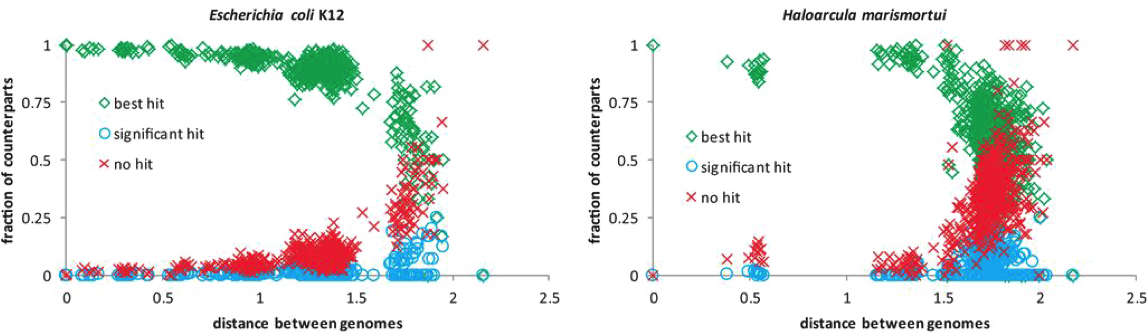
\includegraphics[width=1\textwidth]{images/syntenic_triplet_results} 
  \end{center}
\end{frame}

% Which methods work best
\begin{frame}
  \frametitle{Which prediction methods work best?
    \footnote{\tiny{Salichos and Rokas (2011) \textit{PLoS One} \textbf{6}:e18755 \href{http://dx.doi.org/10.1371/journal.pone.0018755.g006}{doi:10.1371/journal.pone.0018755.g006
  }}}
  }
  Four methods tested against 2,723 curated orthologues from six \textit{Saccharomycetes}
  \begin{itemize}
    \item \textcolor{hutton_green}{RBBH (and cRBH); RSD (and cRSD); MultiParanoid; OrthoMCL}
    \item \textcolor{hutton_blue}{Rated by statistical performance metrics: sensitivity, specificity, accuracy, FDR}
  \end{itemize}
  \textcolor{hutton_purple}{\textbf{cRBH most accurate and specific, with lowest FDR.}}
  \begin{center}
      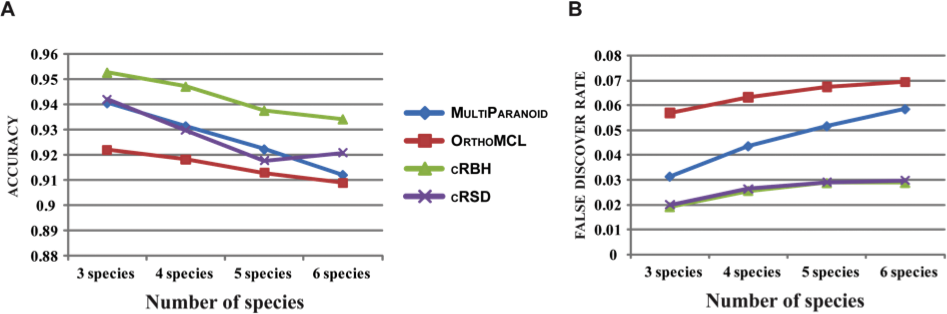
\includegraphics[height=0.25\textheight]{images/salichos_results1} 
      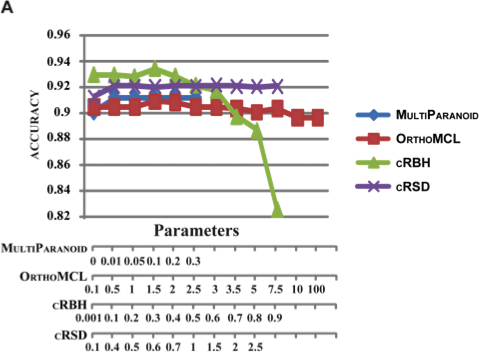
\includegraphics[height=0.25\textheight]{images/salichos_results2}      
  \end{center}
\end{frame}

% Which methods work best
\begin{frame}
  \frametitle{Which prediction methods work best?
    \footnote{\tiny{Altenhoff and Dessimoz (2009) \textit{PLoS Comp. Biol.} \textbf{5}:e1000262 \href{http://dx.doi.org/10.1371/journal.pcbi.1000262}{doi:10.1371/journal.pcbi.1000262
    }}}
  }
  Testing on literature-based benchmarks for grouping by function and correct branching of phylogeny.  \begin{center}
      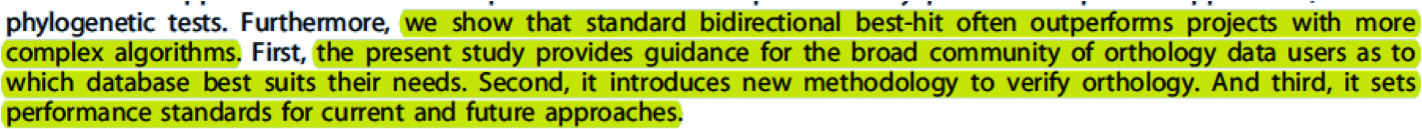
\includegraphics[width=1\textwidth]{images/altenhoff1} \\
      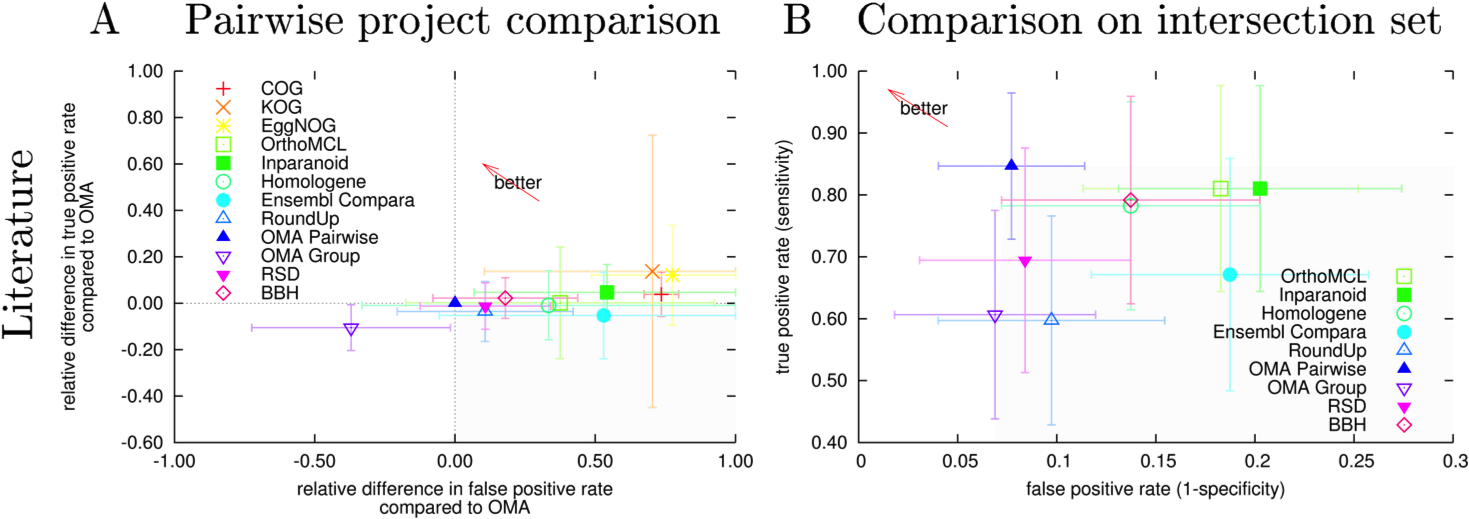
\includegraphics[width=1\textwidth]{images/altenhoff2}      
  \end{center}
\end{frame}

% Which methods work best
\begin{frame}
  \frametitle{Which prediction methods work best?}
  \begin{itemize}
    \item \textcolor{hutton_green}{Performance varies by choice of method, and interpretation of ``orthology''}
    \item \textcolor{hutton_blue}{Biggest influence is genome annotation quality}
    \item Relative performance varies with choice of benchmark
    \item \textcolor{hutton_purple}{\textbf{(clustering) RBH outperforms more complex algorithms under many circumstances}}
  \end{itemize}
\end{frame}

% Which methods work best
\begin{frame}
  \frametitle{What is this magic RBH method?}
  \begin{center}
      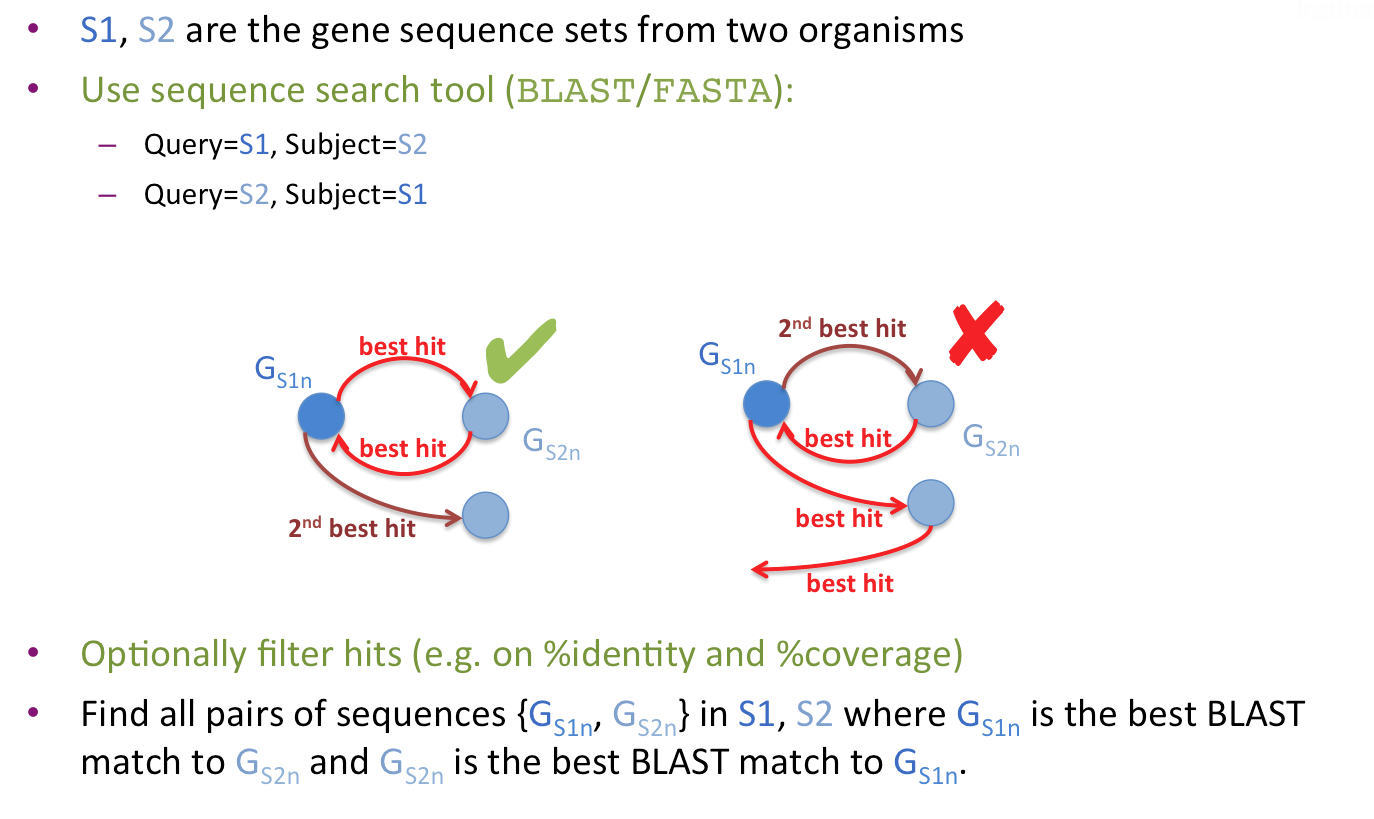
\includegraphics[width=1\textwidth]{images/rbbh}      
  \end{center}
\end{frame}

%
\begin{frame}
  \frametitle{Finding ``Orthologues'': RBBH}
  \Large{
    \textcolor{hutton_blue}{
      \textbf{
      EXERCISE 8: \\
      \texttt{ex08\_find\_rbbh.ipynb}
      }
    }
  }
\end{frame}

%
\begin{frame}
  \frametitle{Finding ``Orthologues'': MCL}
  \Large{
    \textcolor{hutton_blue}{
      \textbf{
      EXERCISE 9: \\
      {\small \href{https://github.com/widdowquinn/Teaching-2015-03-17-UoD_compgenvis/blob/master/exercises/mcl_orthologues/ex09_mcl_orthologues.md}{\texttt{mcl\_orthologues/ex\_09a\_mcl\_orthologues.md}} \\
      \texttt{mcl\_orthologues/ex09b\_mcl\_orthologues.ipynb}}
      }
    }
  }
\end{frame}
%% using_orthologue_prediction.tex
%% Author: Leighton Pritchard
%% Copyright: James Hutton Institute
%% A brief introduction to orthologues, and evaluation of their prediction

% SUBSECTION: Why orthologues?
\subsection{Using orthologue predictions}

% Which methods work best
\begin{frame}
  \frametitle{Functional adaptation in \textit{Pba}\footnote{\tiny{Toth \textit{et al}. (2006) \textit{Ann. Rev. Phytopath.} \textbf{44}:305-336 \href{http://dx.doi.org/10.1146/annurev.phyto.44.070505.143444}{doi:10.1146/annurev.phyto.44.070505.143444}}}}
  \begin{center}
      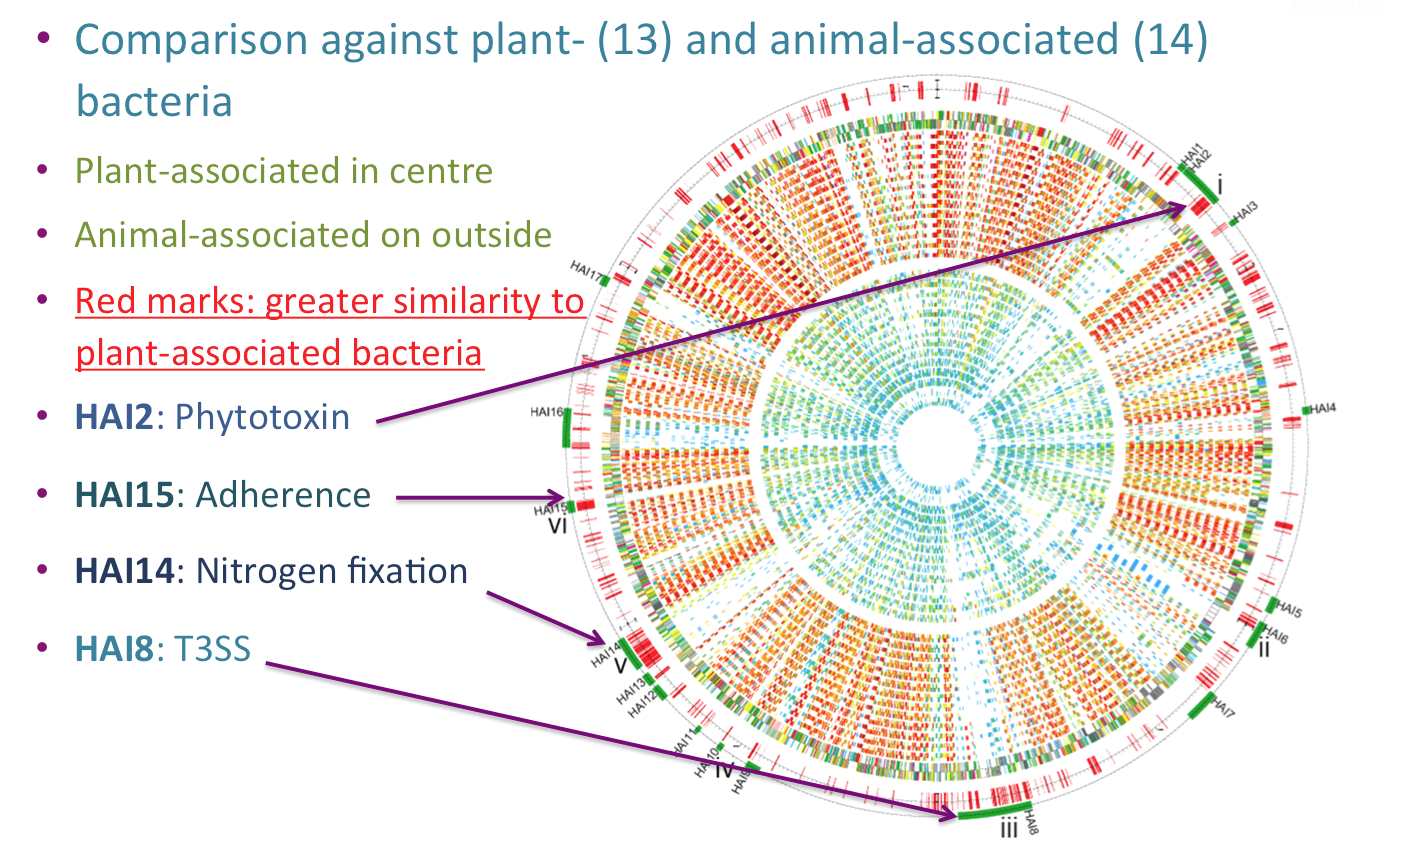
\includegraphics[width=1\textwidth]{images/pba_lgt} 
  \end{center}
\end{frame}

% Which methods work best
\begin{frame}
  \frametitle{Functional adaptation in \textit{Pba}\footnote{\tiny{Toth \textit{et al}. (2006) \textit{Ann. Rev. Phytopath.} \textbf{44}:305-336 \href{http://dx.doi.org/10.1146/annurev.phyto.44.070505.143444}{doi:10.1146/annurev.phyto.44.070505.143444}}}}
  \begin{center}
      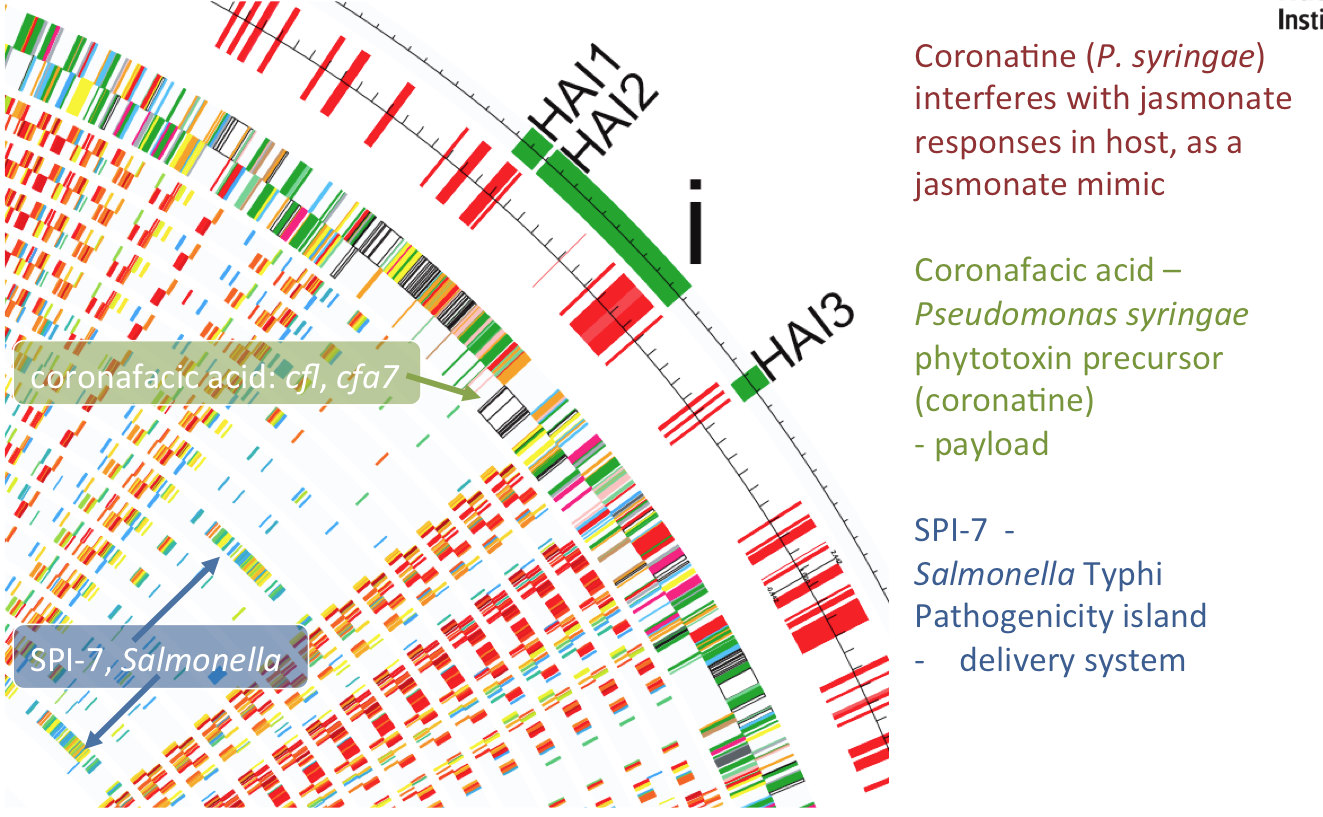
\includegraphics[width=1\textwidth]{images/pba_coronatine} 
  \end{center}
\end{frame}

% SUBSECTION: Core and pangenomes
\subsection{Core and Pan-genomes}

% Which methods work best
\begin{frame}
  \frametitle{Core genome}
  Once equivalent genes have been identified, those present in all related isolates can be identified: \textbf{\textit{the core genome}}.\\
  The \textit{core} genome is expected to underpin common function.\\
  A core RBH cluster (\textit{clique}) for 29 genomes:
  \begin{center}
      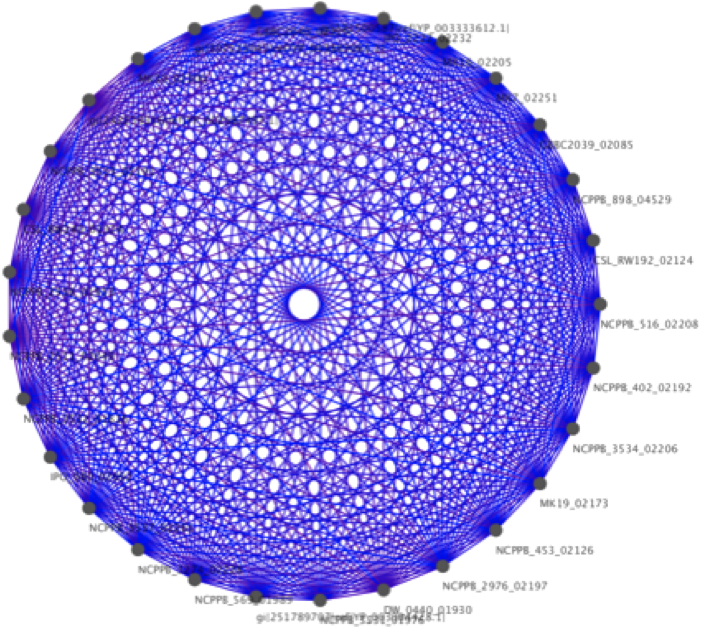
\includegraphics[height=0.55\textheight]{images/core_cluster} 
  \end{center}
\end{frame}

% Which methods work best
\begin{frame}
  \frametitle{Accessory genome}
  The remaining genes are \textbf{\textit{the accessory genome}}, and are expected to mediate function that distinguishes between isolates.\\[0.2cm]
  An accessory RBH cluster for 29 genomes:
  \begin{center}
      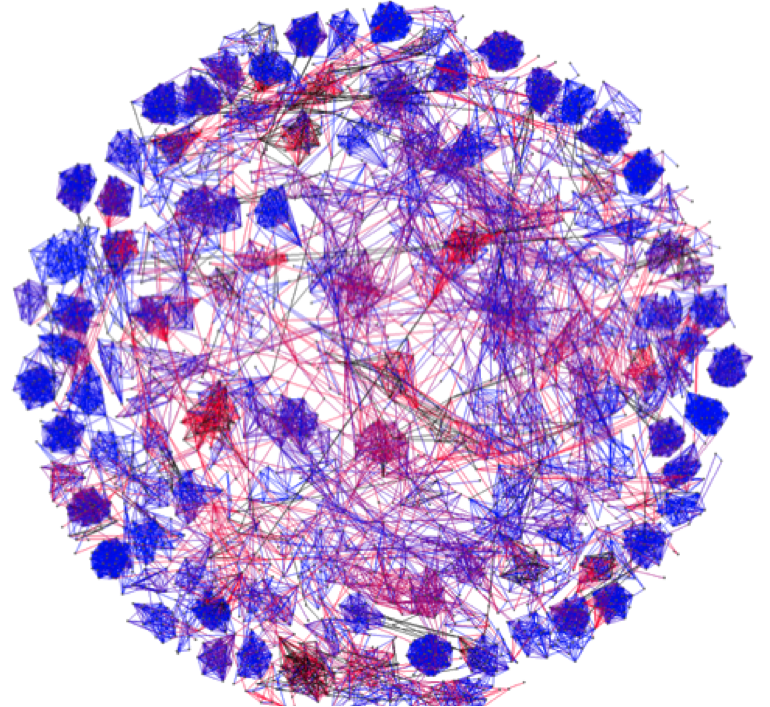
\includegraphics[height=0.5\textheight]{images/accessory_cluster} 
  \end{center}
\end{frame}

% Which methods work best
\begin{frame}
  \frametitle{Accessory clusters}
  Accessory RBH clusters can be pruned, to identify the accessory genome specific to subgroups of isolates:
  \begin{center}
      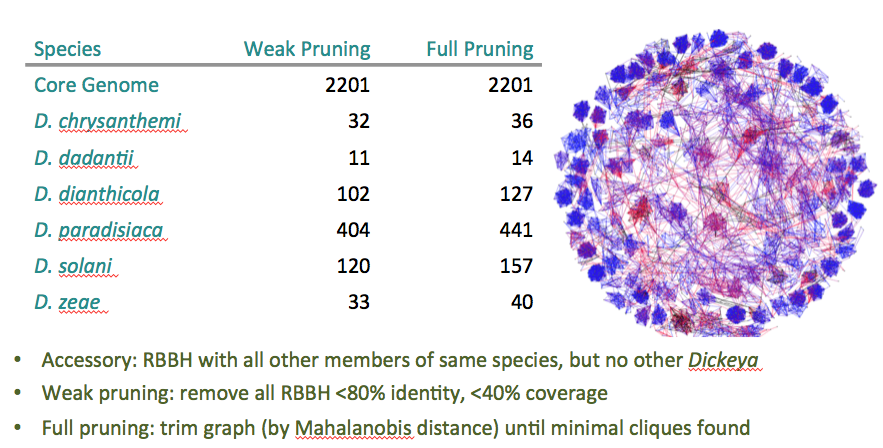
\includegraphics[height=0.55\textheight]{images/dickeya_accessory} 
  \end{center}
  These genes may be responsible for subgroup-specific phenotypes
\end{frame}

% Which methods work best
\begin{frame}
  \frametitle{Accessory genome
   \footnote{\tiny{Croll and Mcdonald (2012) \textit{PLoS Path.} \textbf{8}:e1002608 \href{http://dx.doi.org/10.1371/journal.ppat.1002608}{doi:10.1371/journal.ppat.1002608
  }}}
    \footnote{\tiny{Baltrus \textit{et al}. (2011) \textit{PLoS Path.} \textbf{7}:e1002132 \href{http://dx.doi.org/10.1371/journal.ppat.1002132.t002}{doi:10.1371/journal.ppat.1002132.t002
    }}}  
  }
  Accessory genomes act as a cradle for adaptive evolution \\[0.2cm]
  This is particularly so for bacterial pathogens, such as \textit{Pseudomonas} spp.
  \begin{center}
      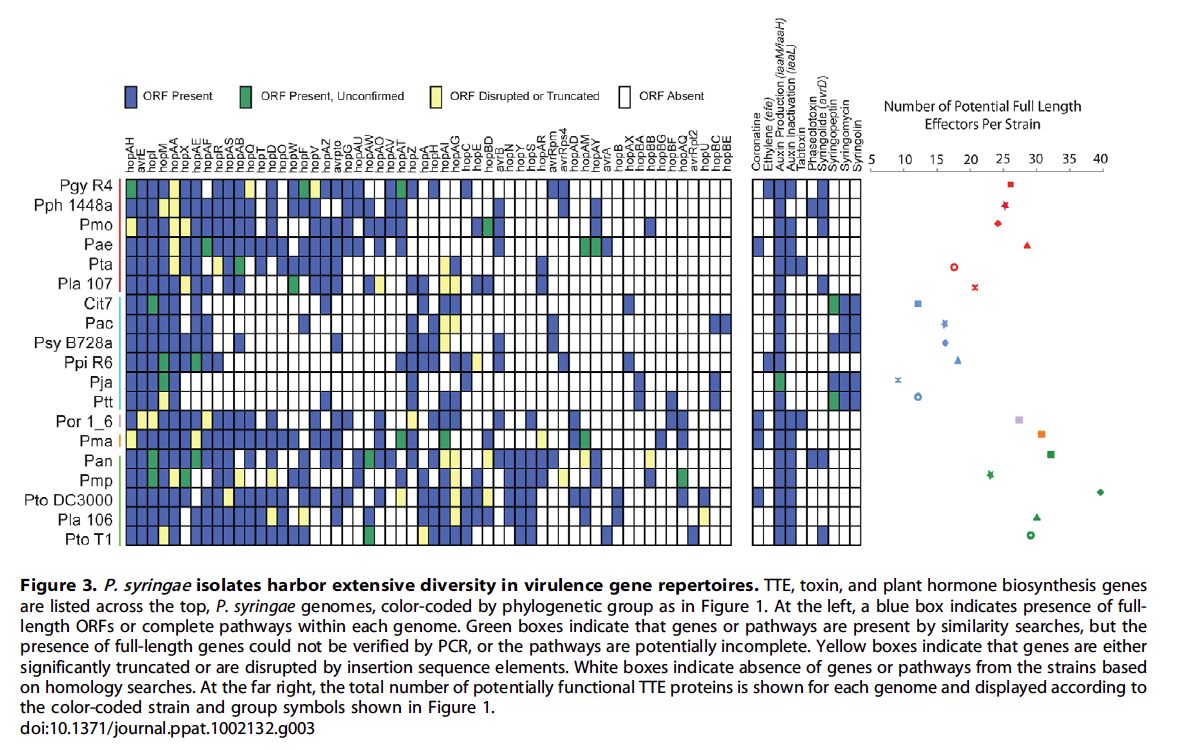
\includegraphics[height=0.5\textheight]{images/pa_virulence} 
  \end{center}
\end{frame}

% Which methods work best
\begin{frame}
  \frametitle{Core genome synteny
    \footnote{\tiny{Proost \textit{et al}. (2012) \textit{Nuc. Acids Res.} \textbf{40}:e11 \href{http://dx.doi.org/10.1093/nar/gkr955}{doi:10.1093/nar/gkr955
    }}}
  }
  Using tools like i-ADHoRe that identify synteny and collinearity, the structural organisation of the core genome can be determined:
  \begin{center}
      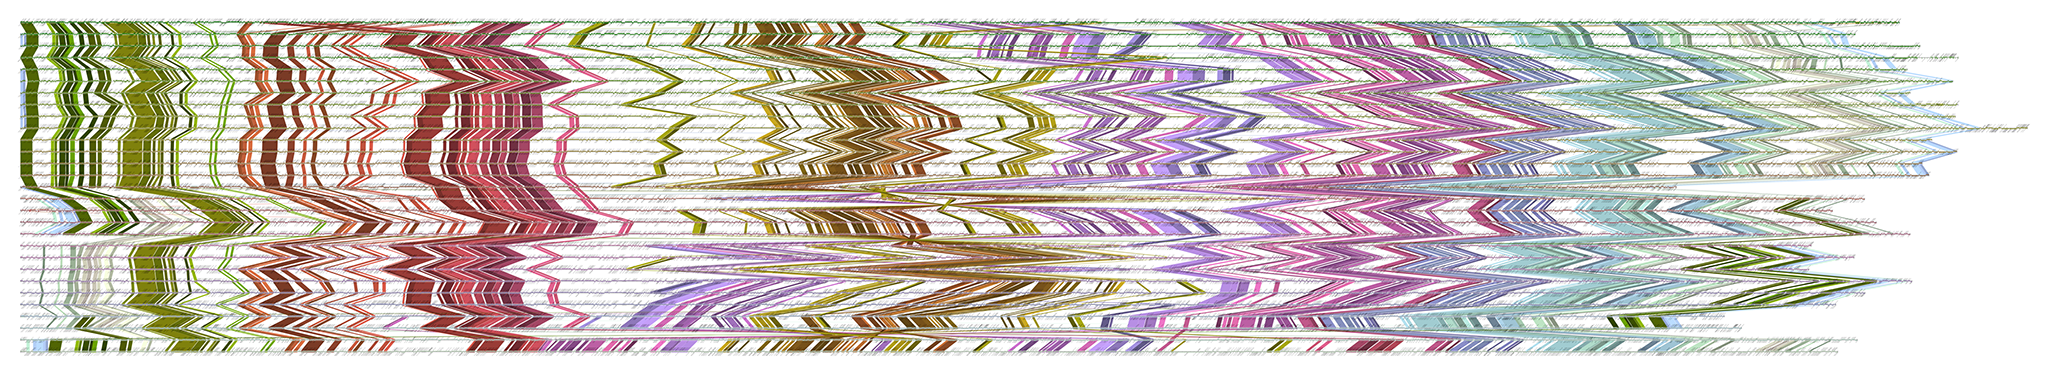
\includegraphics[width=1\textwidth]{images/dickeya_core_collinear_small} 
  \end{center}
  For \textit{Dickeya}, the core genome appears to be structurally well-conserved across all isolates.
\end{frame}

% Which methods work best
\begin{frame}
  \frametitle{Panseq\footnote{\tiny{Laing \textit{et al}. (2010) \textit{BMC Bioinf.} \textbf{11}:461 \href{http://dx.doi.org/10.1186/1471-2105-11-461}{doi:10.1186/1471-2105-11-461}}}}
  \texttt{Panseq} is an online tool for identification of core and accessory genomes, available at \href{https://lfz.corefacility.ca/panseq/}{https://lfz.corefacility.ca/panseq/}, and \href{https://github.com/chadlaing/Panseq}{https://github.com/chadlaing/Panseq} for standalone use
  \begin{center}
      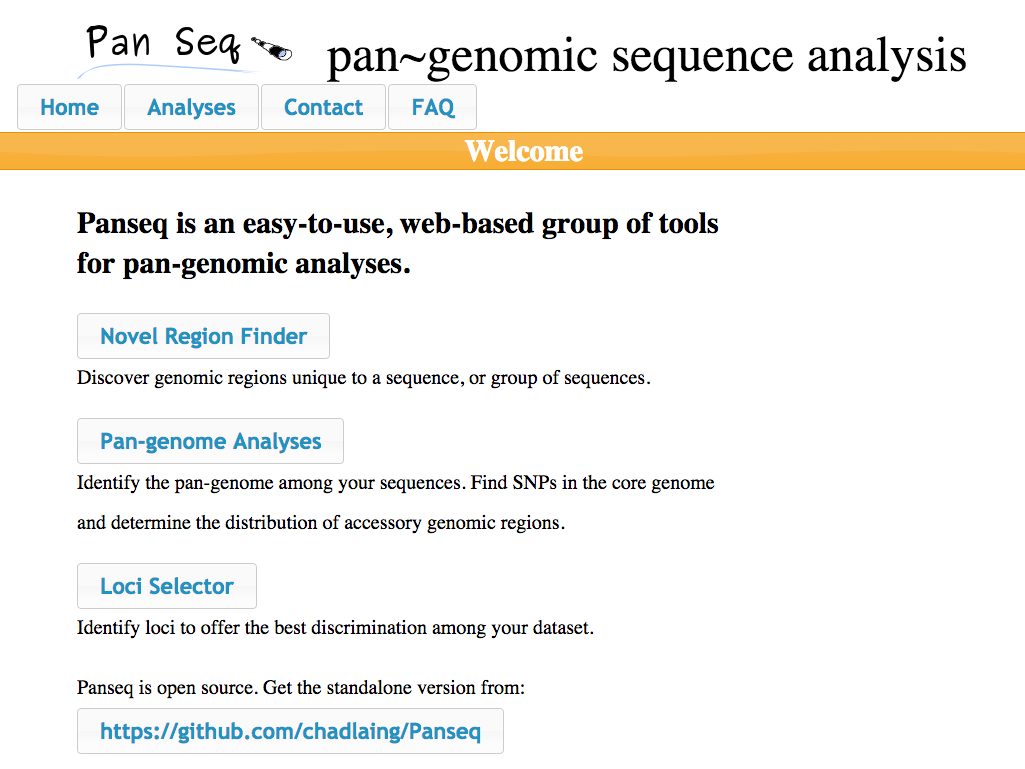
\includegraphics[width=0.7\textwidth]{images/panseq} 
  \end{center}
\end{frame}

%
\begin{frame}
  \frametitle{Harvest\footnote{\tiny{Treangen \textit{et al}. (2014) \textit{Genome Biol.} \textbf{15}:524 \href{http://dx.doi.org/10.1186/s13059-014-0524-x}{doi:10.1186/s13059-014-0524-x}}}}
  Visualising and organising comparison/pangenome data across thousands of bacteria is difficult.\\
  \textit{Very} recently (this week), the \texttt{Harvest} suite of tools was published, for alignment and visualisation of thousands of genomes:
  \begin{center}
      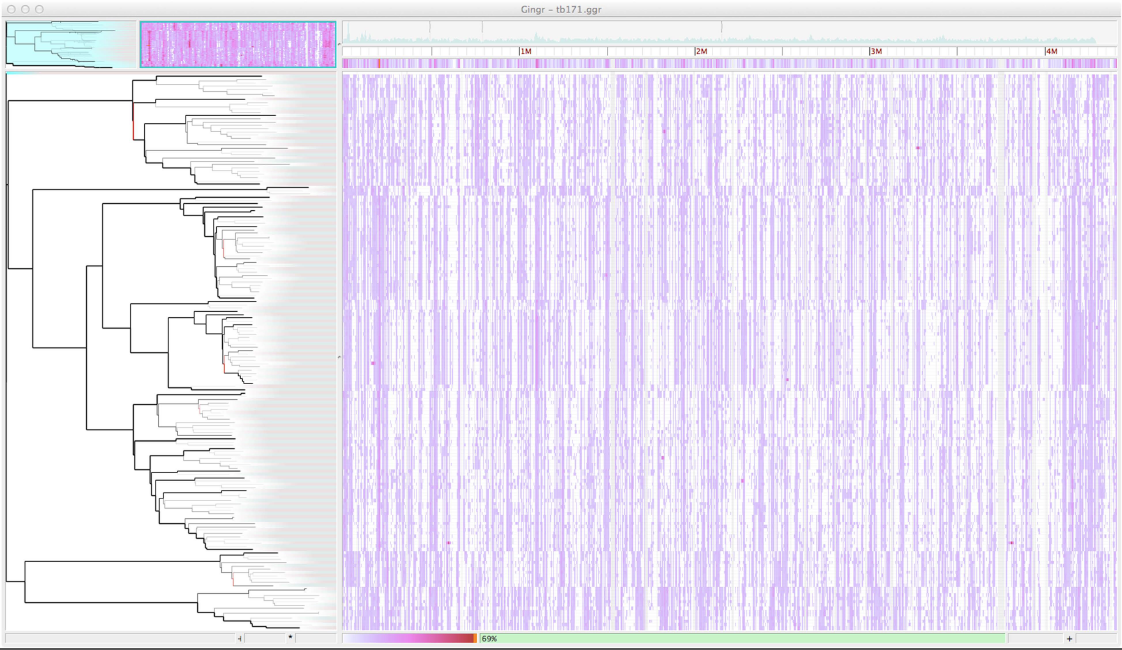
\includegraphics[width=0.8\textwidth]{images/harvest} 
  \end{center}
\end{frame}


% SUBSECTION
% Selection Pressure
\subsection{Selection Pressure}
%% selection_pressure.tex
%% Author: Leighton Pritchard
%% Copyright: James Hutton Institute
%% A brief introduction to orthologues, and their prediction

%
\begin{frame}
  \frametitle{Selection Pressure
  }
  \Large{
    \textcolor{olive}{
      \textbf{
      Comparative genomics helps identify selection pressures at a structural and sequence level
      }
    }
  }
\end{frame}

%
\begin{frame}
  \frametitle{How orthologues help}
  \textcolor{hutton_green}{Defining core groups of genes as ``orthologue`'' allows analysis of groups of genes together by:}
  \begin{itemize}
    \item \textcolor{hutton_purple}{synteny/collocation}
    \item gene neighbourhood changes (e.g. \textcolor{hutton_purple}{\textit{genome expansion}})
    \item \textcolor{hutton_purple}{pan genome (core/accessory genomes)}
  \end{itemize}
  \textcolor{hutton_blue}{and of individual genes within those groups, by:}
  \begin{itemize}
    \item multiple alignment
    \item domain detection
    \item identification of functional sites
    \item \textcolor{hutton_purple}{inference of evolutionary pressure}
  \end{itemize}  
\end{frame}

%
\begin{frame}
  \frametitle{Synteny
    \footnote{\tiny{Alvarez-Ponce \textit{et al}. (2011) \textit{Genome Biol. Evol.} \href{http://dx.doi.org/10.1093/gbe/evq084}{doi:10.1093/gbe/evq084
  }}}
}
  Selection pressures depend on gene (product) function
  \begin{itemize}
    \item \textcolor{hutton_green}{Genes involving physically or functionally-interacting proteins tend to involve under selective constraints} \\
    In bacteria, this leads to coexpression in \textit{regions} and collocation in \textit{operons}
    \item \textcolor{hutton_blue}{Collocation (and correlation) may be identified by genome comparisons}
    \item \textcolor{RawSienna}{Also true for regulatory and metabolic networks}
  \end{itemize}  
\end{frame}

%
\begin{frame}
  \frametitle{Synteny
    \footnote{\tiny{Soderlund \textit{et al}. (2011) \textit{Nucl. Acids Res.} \href{http://dx.doi.org/10.1093/nar/gkr123}{doi:10.1093/nar/gkr123
  }}}
    \footnote{\tiny{Proost \textit{et al}. (2011) \textit{Nucl. Acids Res.} \href{http://dx.doi.org/10..1093/nar/gkr955}{doi:1093/nar/gkr955
  }}}
}
  Several tools for synteny detection, e.g.
  \begin{columns}[T] 
    \column{.6\textwidth}   
      \begin{itemize}
        \item \textcolor{hutton_green}{SyMAP {\tiny\href{http://www.agcol.arizona.edu/software/symap/}{http://www.agcol.arizona.edu/software/symap/}}}
        \item \textcolor{hutton_blue}{i-ADHoRe {\tiny\href{http://bioinformatics.psb.ugent.be/software/details/i-ADHoRe}{http://bioinformatics.psb.ugent.be/software/details/i-ADHoRe}}}
        \item MCScan, Cyntenator, etc.  
      \end{itemize}  
      \column{.4\textwidth}
        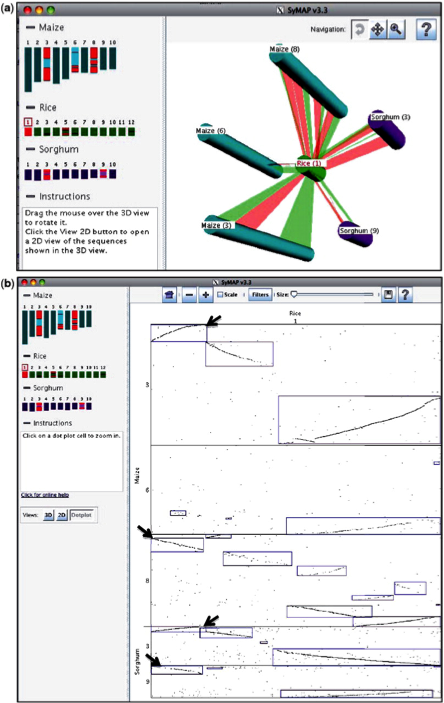
\includegraphics[height=0.6\textheight]{images/symap}
    \end{columns}
\end{frame}

%
\begin{frame}
  \frametitle{i-ADHoRe
    \footnote{\tiny{Proost \textit{et al}. (2011) \textit{Nucl. Acids Res.} \href{http://dx.doi.org/10..1093/nar/gkr955}{doi:1093/nar/gkr955
  }}}
}
  Algorithm: starts from defined equivalent genes to produce genome-scale multiple alignments of blocks of genes
  {\small
  \begin{columns}[T] 
    \column{.4\textwidth}   
      \begin{enumerate}
        \item Combine tandem repeats of gene sets
        \item Make \textcolor{hutton_green}{\textit{gene homology matrix} (GHM)}
        \item Convert collinear GHMs to \textcolor{hutton_blue}{\textit{profiles}}
        \item Align \textit{profiles} (GG2 algorithm)
        \item Search next genome with profiles, and \textcolor{hutton_purple}{iterate until complete}
      \end{enumerate}  
      \column{.6\textwidth}
        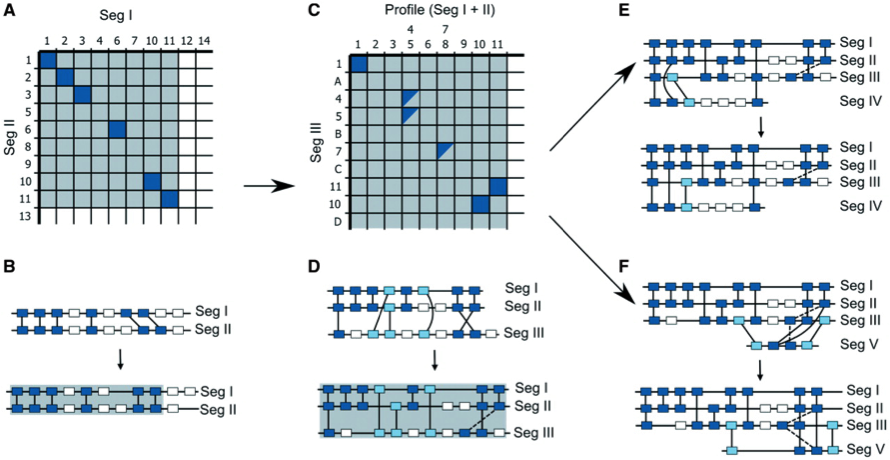
\includegraphics[width=\textwidth]{images/i-adhore_algorithm}
    \end{columns}
    }    
\end{frame}

%
\begin{frame}
  \frametitle{Finding ``Orthologues'': RBBH}
  \Large{
    \textcolor{hutton_blue}{
      \textbf{
      EXERCISE 10: \\
      \texttt{i-ADHoRe/ex10a\_i-ADHoRe.md}      
      \texttt{i-ADHoRe/ex10b\_i-ADHoRe.ipynb}
      }
    }
  }
\end{frame}
%% pangenome.tex
%% Author: Leighton Pritchard
%% Copyright: James Hutton Institute
%% A brief introduction to pangenomes

% Which methods work best
\begin{frame}
  \frametitle{Core genome}
  Once equivalent genes have been identified, those present in all related isolates can be identified: \textbf{\textit{the core genome}}.\\
  \textcolor{hutton_green}{The \textit{core} genome is expected to underpin common function.}\\
  A core RBH cluster (\textit{clique}) for 29 genomes:
  \begin{center}
      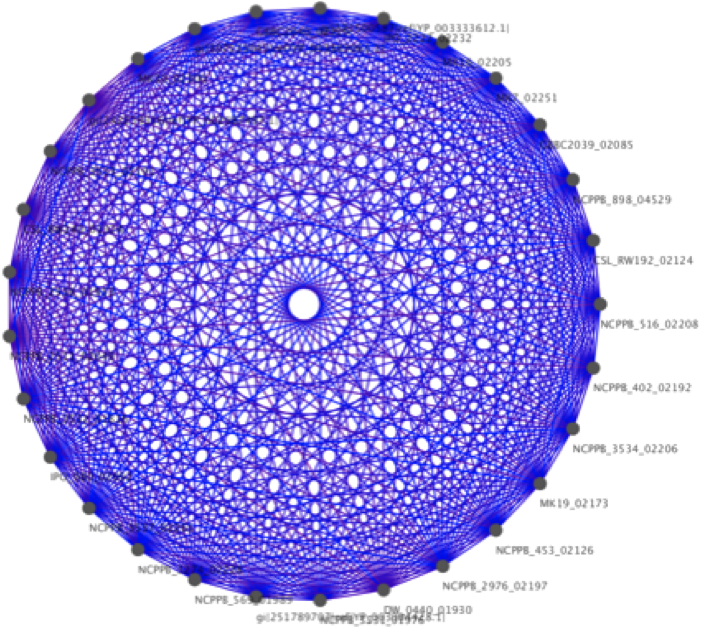
\includegraphics[height=0.55\textheight]{images/core_cluster} 
  \end{center}
\end{frame}

% Which methods work best
\begin{frame}
  \frametitle{Accessory genome}
  \textcolor{hutton_green}{The remaining genes are \textbf{\textit{the accessory genome}}, and are expected to mediate function that distinguishes between isolates.}\\[0.2cm]
  An accessory RBH cluster for 29 genomes:
  \begin{center}
      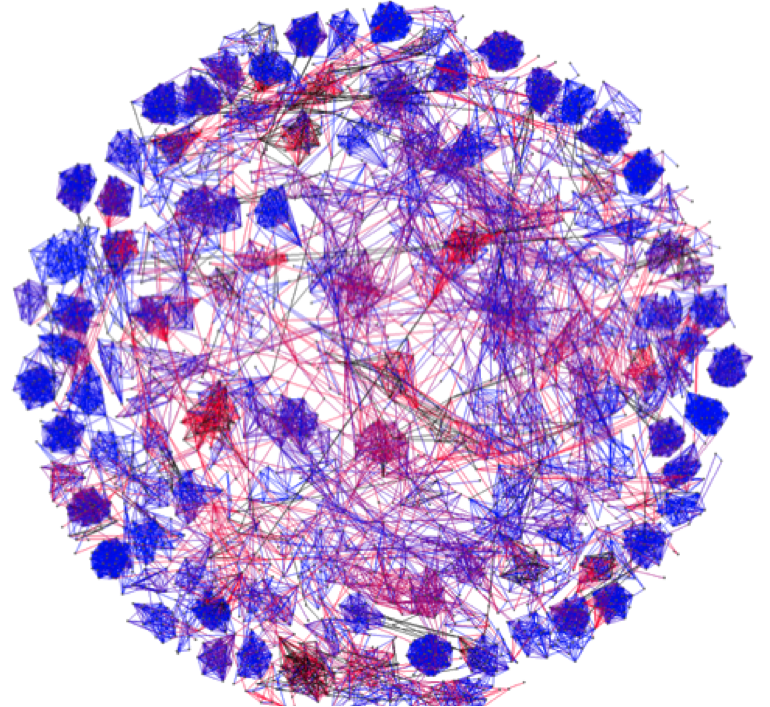
\includegraphics[height=0.5\textheight]{images/accessory_cluster} 
  \end{center}
\end{frame}

% Which methods work best
\begin{frame}
  \frametitle{Accessory clusters}
  Accessory RBH clusters can be pruned, to identify the accessory genome specific to subgroups of isolates:
  \begin{center}
      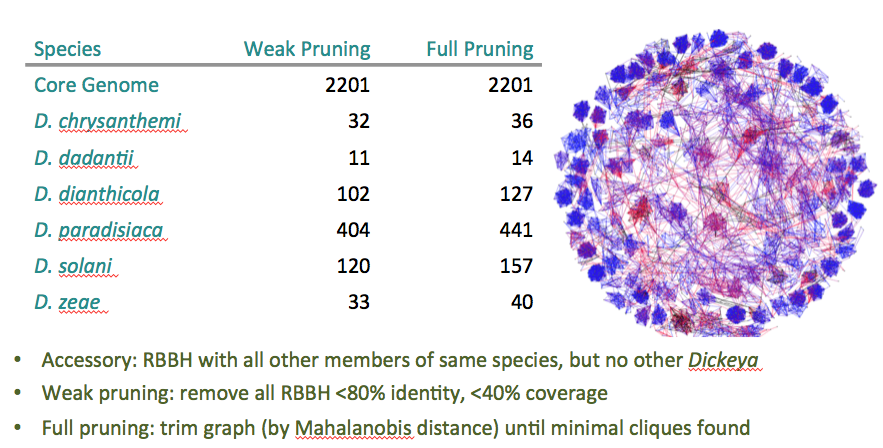
\includegraphics[height=0.55\textheight]{images/dickeya_accessory} 
  \end{center}
  \textcolor{hutton_green}{These genes may be responsible for subgroup-specific phenotypes}
\end{frame}

% Which methods work best
\begin{frame}
  \frametitle{Accessory genome
   \footnote{\tiny{Croll and Mcdonald (2012) \textit{PLoS Path.} \textbf{8}:e1002608 \href{http://dx.doi.org/10.1371/journal.ppat.1002608}{doi:10.1371/journal.ppat.1002608
  }}}
    \footnote{\tiny{Baltrus \textit{et al}. (2011) \textit{PLoS Path.} \textbf{7}:e1002132 \href{http://dx.doi.org/10.1371/journal.ppat.1002132.t002}{doi:10.1371/journal.ppat.1002132.t002
    }}}  
  }
  Accessory genomes are a cradle for adaptive evolution \\
  \textcolor{hutton_green}{This is particularly so for bacterial pathogens, such as \textit{Pseudomonas} spp.}
  \begin{center}
      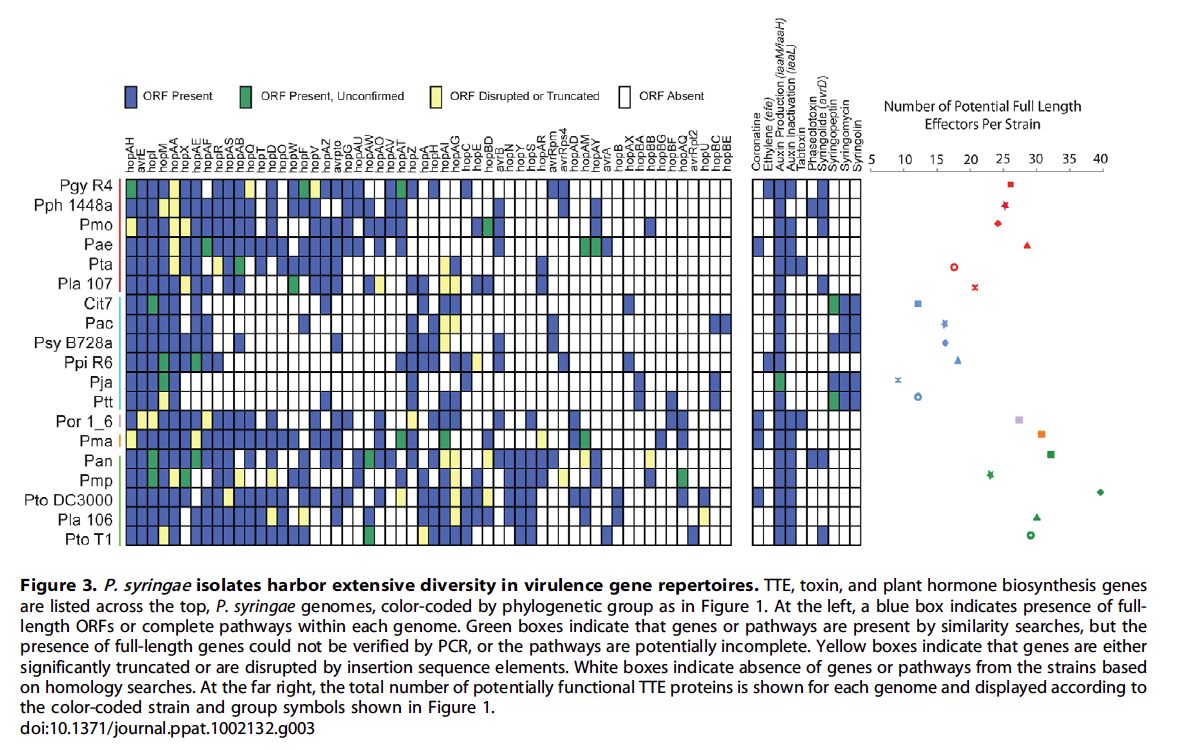
\includegraphics[height=0.5\textheight]{images/pa_virulence} 
  \end{center}
\end{frame}

% Which methods work best
\begin{frame}
  \frametitle{Core genome synteny
    \footnote{\tiny{Proost \textit{et al}. (2012) \textit{Nuc. Acids Res.} \textbf{40}:e11 \href{http://dx.doi.org/10.1093/nar/gkr955}{doi:10.1093/nar/gkr955
    }}}
  }
  Using tools like i-ADHoRe that identify synteny and collinearity, the structural organisation of the core genome can be determined:
  \begin{center}
      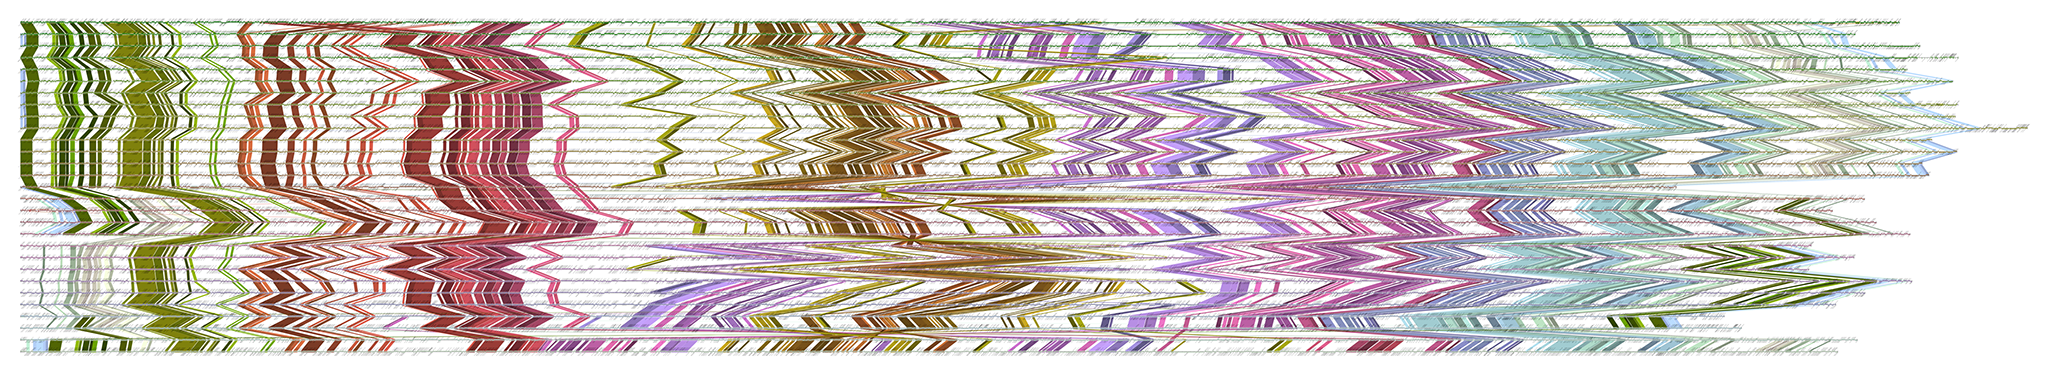
\includegraphics[width=1\textwidth]{images/dickeya_core_collinear_small} 
  \end{center}
  For \textit{Dickeya}, the core genome appears to be structurally well-conserved across all isolates.
\end{frame}

% Which methods work best
\begin{frame}
  \frametitle{Panseq
  \footnote{\tiny{Laing \textit{et al}. (2010) \textit{BMC Bioinf.} \textbf{11}:461 \href{http://dx.doi.org/10.1186/1471-2105-11-461}{doi:10.1186/1471-2105-11-461
  }}}
  \footnote{\tiny{\href{https://lfz.corefacility.ca/panseq/}{https://lfz.corefacility.ca/panseq/
  }}}  }
  \texttt{Panseq} is a tool for identification of core and accessory genomes
  \begin{center}
      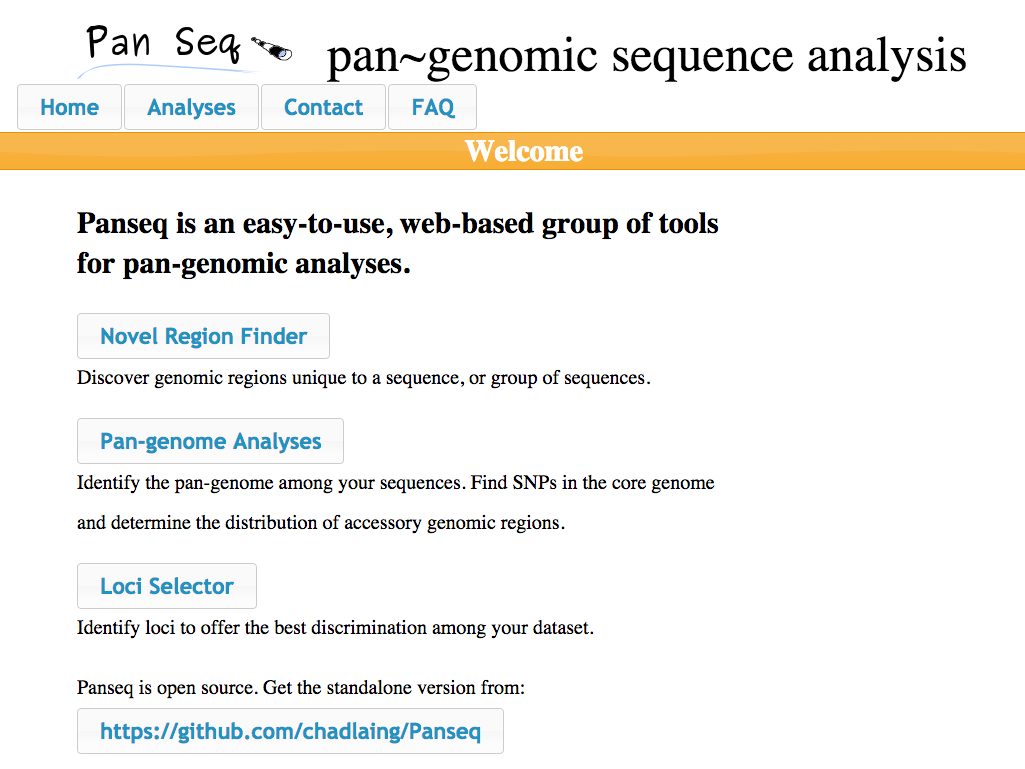
\includegraphics[width=0.7\textwidth]{images/panseq} 
  \end{center}
\end{frame}

%
\begin{frame}
  \frametitle{Harvest
  \footnote{\tiny{Treangen \textit{et al}. (2014) \textit{Genome Biol.} \textbf{15}:524 \href{http://dx.doi.org/10.1186/s13059-014-0524-x}{doi:10.1186/s13059-014-0524-x
  }}}
  }
  \textcolor{hutton_green}{Visualising and organising comparison/pangenome data across thousands of bacteria is difficult.}\\
  \texttt{Harvest} suite of tools, for alignment and visualisation of thousands of genomes:
  \begin{center}
      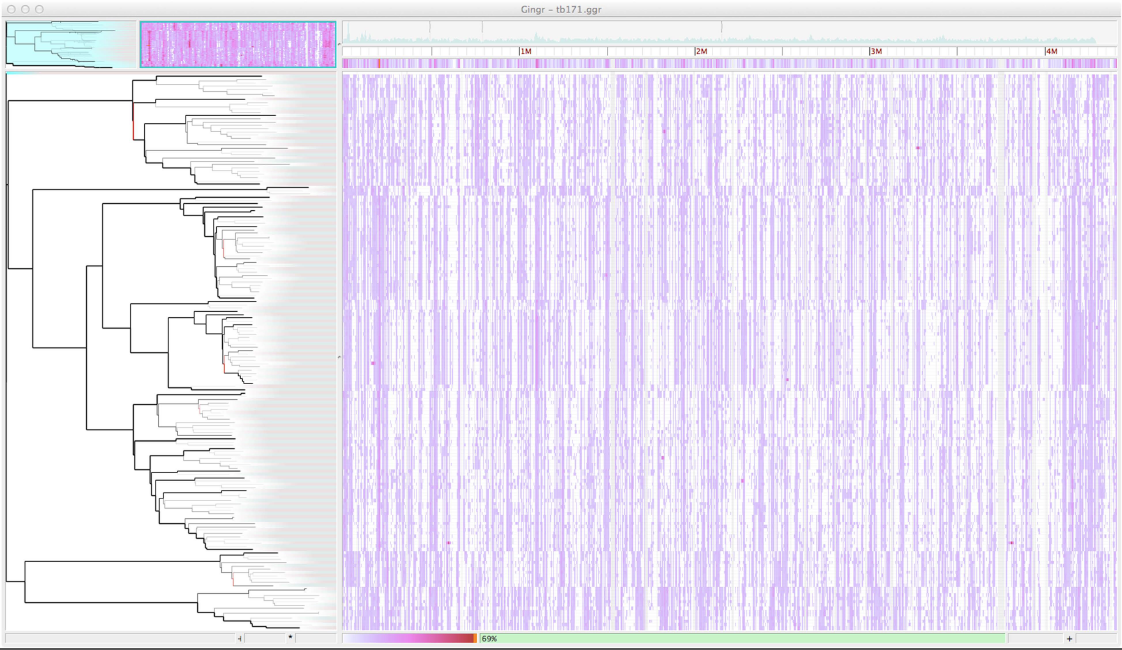
\includegraphics[width=0.8\textwidth]{images/harvest} 
  \end{center}
\end{frame}

% SUBSECTION
% Finishing the Hat
\subsection{Finishing the Hat}
%% final_slides.tex
%% Author: Leighton Pritchard
%% Copyright: James Hutton Institute
%% Final slides

%
\begin{frame}
  \frametitle{What didn't I get to?}
  \begin{itemize}
    \item   \textcolor{hutton_green}{Genome-Wide Association Studies (GWAS)}
    \begin{itemize}
      \item   Try \href{http://genenetwork.org/}{http://genenetwork.org/} to play with some data
    \end{itemize}
    \item Prediction of regulatory elements, e.g.
    \begin{itemize}
      \item {\tiny\href{http://dx.doi.org/10.1038/nature01644}
                              {Kellis \textit{et al.} (2003) \textit{Nature} doi:10.1038/nature01644}}
      \item {\tiny\href{http://dx.doi.org/10.1101/gr.5592107}
                              {King \textit{et al.} (2007) \textit{Genome Res.} doi:10.1101/gr.5592107}}
      \item {\tiny\href{http://dx.doi.org/10.1186/1471-2105-9-455}
                              {Chaivorapol \textit{et al.} (2008) \textit{BMC Bioinf.} doi:10.1186/1471-2105-9-455}}
      \item {\tiny\href{http://genome.ucsf.edu/compmoby}
                              {CompMOBY http://genome.ucsf.edu/compmoby}}
    \end{itemize}
    \item   \textcolor{hutton_purple}{Detection of Horizontal/Lateral Gene Transfer (HGT/LGT), e.g.}
    \begin{itemize}
      \item {\tiny\href{http://dx.doi.org/10.1093/nar/gki187}
                              {Tsirigos \& Rigoutsos (2005) \textit{Nucl. Acids Res.} doi:10.1093/nar/gki187}}
    \end{itemize}
    \item   \textcolor{RawSienna}{Phylogenomics, e.g.}
    \begin{itemize}
      \item {\tiny\href{http://dx.doi.org/10.1038/nrg1603}
                              {Delsuc \textit{et al.} (2005) \textit{Nat. rev. Genet.} doi:10.1038/nrg1603}}
      \item {\tiny\href{https://phylogenomics.wordpress.com/software/amphora/}
                              {AMPHORA https://phylogenomics.wordpress.com/software/amphora/}}
    \end{itemize}
  \end{itemize}
\end{frame}

\begin{frame}
  \frametitle{Messages to take away}
  \begin{itemize}
    \item   \textcolor{hutton_green}{Comparative genomics is a powerful set of techniques for:}
    \begin{itemize}
      \item Understanding and identifying evolutionary processes and mechanisms
      \item Reconstructing detailed evolutionary history of a set of organisms
      \item Identifying and understanding common genomic features of organisms
      \item Providing hypotheses about gene function for experimental investigation
    \end{itemize}
  \end{itemize}
\end{frame}

\begin{frame}
  \frametitle{Messages to take away}
  \begin{itemize}
    \item \textcolor{hutton_blue}{A huge amount of data is available to work with}
    \begin{itemize}
      \item And it's only going to get much, much larger
    \end{itemize}
    \item \textcolor{hutton_purple}{Results feed into many areas of study:}
    \begin{itemize}
      \item Medicine and health
      \item Agriculture and food security
      \item Basic biology in all fields
      \item Systems and synthetic biology
    \end{itemize}
  \end{itemize}
\end{frame}

\begin{frame}
  \frametitle{Messages to take away}
  \begin{itemize}
    \item \textcolor{hutton_green}{Comparative genomics is comparisons}
    \begin{itemize}
      \item What is \textit{similar} between two genomes?
      \item What is \textit{different} between two genomes?
    \end{itemize}
    \item \textcolor{hutton_blue}{Comparative genomics \textit{is} evolutionary genomics}
    \begin{itemize}
      \item Lots of scope for improvement in tools
    \end{itemize}
    \item \textcolor{hutton_purple}{Tools that `do the same thing' can give different output}
    \begin{itemize}
      \item BLAST vs MUMmer
      \item RBBH vs MCL
      \item The choice of application matters for correctness and interpretation
    \end{itemize}
  \end{itemize}
\end{frame}

\begin{frame}
  \frametitle{Messages to take away}
  Comparative genomics is
  \begin{itemize}
    \item \textcolor{hutton_green}{Fun}
    \item \textcolor{hutton_blue}{Indoor work, in the warm and dry}
    \item \textcolor{hutton_purple}{Not a job that involves a lot of heavy lifting}
  \end{itemize}
\end{frame}

%%%
% LICENCE FOR REUSE
%% licence.tex
%% Author: Leighton Pritchard
%% Copyright: James Hutton Institute
%% These slides describe the licence for reuse of these slides and
%% materials

%
\begin{frame}
  \frametitle{Licence: CC-BY-SA}
  By: Leighton Pritchard \\[0.5cm]
  This presentation is licensed under the Creative Commons Attribution ShareAlike license \\
  \href{https://creativecommons.org/licenses/by-sa/4.0/}{https://creativecommons.org/licenses/by-sa/4.0/}
\end{frame}

% etc
\end{document}